\documentclass{article} % For LaTeX2e
\usepackage{icomp2024_conference,times}

% Optional math command from https://github.com/goodfeli/dlbook_notation.
%%%%% NEW MATH DEFINITIONS %%%%%

\usepackage{amsmath,amsfonts,bm}

% Mark sections of captions for referring to divisions of figures
\newcommand{\figleft}{{\em (Left)}}
\newcommand{\figcenter}{{\em (Center)}}
\newcommand{\figright}{{\em (Right)}}
\newcommand{\figtop}{{\em (Top)}}
\newcommand{\figbottom}{{\em (Bottom)}}
\newcommand{\captiona}{{\em (a)}}
\newcommand{\captionb}{{\em (b)}}
\newcommand{\captionc}{{\em (c)}}
\newcommand{\captiond}{{\em (d)}}

% Highlight a newly defined term
\newcommand{\newterm}[1]{{\bf #1}}


% Figure reference, lower-case.
\def\figref#1{figure~\ref{#1}}
% Figure reference, capital. For start of sentence
\def\Figref#1{Figure~\ref{#1}}
\def\twofigref#1#2{figures \ref{#1} and \ref{#2}}
\def\quadfigref#1#2#3#4{figures \ref{#1}, \ref{#2}, \ref{#3} and \ref{#4}}
% Section reference, lower-case.
\def\secref#1{section~\ref{#1}}
% Section reference, capital.
\def\Secref#1{Section~\ref{#1}}
% Reference to two sections.
\def\twosecrefs#1#2{sections \ref{#1} and \ref{#2}}
% Reference to three sections.
\def\secrefs#1#2#3{sections \ref{#1}, \ref{#2} and \ref{#3}}
% Reference to an equation, lower-case.
\def\eqref#1{equation~\ref{#1}}
% Reference to an equation, upper case
\def\Eqref#1{Equation~\ref{#1}}
% A raw reference to an equation---avoid using if possible
\def\plaineqref#1{\ref{#1}}
% Reference to a chapter, lower-case.
\def\chapref#1{chapter~\ref{#1}}
% Reference to an equation, upper case.
\def\Chapref#1{Chapter~\ref{#1}}
% Reference to a range of chapters
\def\rangechapref#1#2{chapters\ref{#1}--\ref{#2}}
% Reference to an algorithm, lower-case.
\def\algref#1{algorithm~\ref{#1}}
% Reference to an algorithm, upper case.
\def\Algref#1{Algorithm~\ref{#1}}
\def\twoalgref#1#2{algorithms \ref{#1} and \ref{#2}}
\def\Twoalgref#1#2{Algorithms \ref{#1} and \ref{#2}}
% Reference to a part, lower case
\def\partref#1{part~\ref{#1}}
% Reference to a part, upper case
\def\Partref#1{Part~\ref{#1}}
\def\twopartref#1#2{parts \ref{#1} and \ref{#2}}

\def\ceil#1{\lceil #1 \rceil}
\def\floor#1{\lfloor #1 \rfloor}
\def\1{\bm{1}}
\newcommand{\train}{\mathcal{D}}
\newcommand{\valid}{\mathcal{D_{\mathrm{valid}}}}
\newcommand{\test}{\mathcal{D_{\mathrm{test}}}}

\def\eps{{\epsilon}}


% Random variables
\def\reta{{\textnormal{$\eta$}}}
\def\ra{{\textnormal{a}}}
\def\rb{{\textnormal{b}}}
\def\rc{{\textnormal{c}}}
\def\rd{{\textnormal{d}}}
\def\re{{\textnormal{e}}}
\def\rf{{\textnormal{f}}}
\def\rg{{\textnormal{g}}}
\def\rh{{\textnormal{h}}}
\def\ri{{\textnormal{i}}}
\def\rj{{\textnormal{j}}}
\def\rk{{\textnormal{k}}}
\def\rl{{\textnormal{l}}}
% rm is already a command, just don't name any random variables m
\def\rn{{\textnormal{n}}}
\def\ro{{\textnormal{o}}}
\def\rp{{\textnormal{p}}}
\def\rq{{\textnormal{q}}}
\def\rr{{\textnormal{r}}}
\def\rs{{\textnormal{s}}}
\def\rt{{\textnormal{t}}}
\def\ru{{\textnormal{u}}}
\def\rv{{\textnormal{v}}}
\def\rw{{\textnormal{w}}}
\def\rx{{\textnormal{x}}}
\def\ry{{\textnormal{y}}}
\def\rz{{\textnormal{z}}}

% Random vectors
\def\rvepsilon{{\mathbf{\epsilon}}}
\def\rvtheta{{\mathbf{\theta}}}
\def\rva{{\mathbf{a}}}
\def\rvb{{\mathbf{b}}}
\def\rvc{{\mathbf{c}}}
\def\rvd{{\mathbf{d}}}
\def\rve{{\mathbf{e}}}
\def\rvf{{\mathbf{f}}}
\def\rvg{{\mathbf{g}}}
\def\rvh{{\mathbf{h}}}
\def\rvu{{\mathbf{i}}}
\def\rvj{{\mathbf{j}}}
\def\rvk{{\mathbf{k}}}
\def\rvl{{\mathbf{l}}}
\def\rvm{{\mathbf{m}}}
\def\rvn{{\mathbf{n}}}
\def\rvo{{\mathbf{o}}}
\def\rvp{{\mathbf{p}}}
\def\rvq{{\mathbf{q}}}
\def\rvr{{\mathbf{r}}}
\def\rvs{{\mathbf{s}}}
\def\rvt{{\mathbf{t}}}
\def\rvu{{\mathbf{u}}}
\def\rvv{{\mathbf{v}}}
\def\rvw{{\mathbf{w}}}
\def\rvx{{\mathbf{x}}}
\def\rvy{{\mathbf{y}}}
\def\rvz{{\mathbf{z}}}

% Elements of random vectors
\def\erva{{\textnormal{a}}}
\def\ervb{{\textnormal{b}}}
\def\ervc{{\textnormal{c}}}
\def\ervd{{\textnormal{d}}}
\def\erve{{\textnormal{e}}}
\def\ervf{{\textnormal{f}}}
\def\ervg{{\textnormal{g}}}
\def\ervh{{\textnormal{h}}}
\def\ervi{{\textnormal{i}}}
\def\ervj{{\textnormal{j}}}
\def\ervk{{\textnormal{k}}}
\def\ervl{{\textnormal{l}}}
\def\ervm{{\textnormal{m}}}
\def\ervn{{\textnormal{n}}}
\def\ervo{{\textnormal{o}}}
\def\ervp{{\textnormal{p}}}
\def\ervq{{\textnormal{q}}}
\def\ervr{{\textnormal{r}}}
\def\ervs{{\textnormal{s}}}
\def\ervt{{\textnormal{t}}}
\def\ervu{{\textnormal{u}}}
\def\ervv{{\textnormal{v}}}
\def\ervw{{\textnormal{w}}}
\def\ervx{{\textnormal{x}}}
\def\ervy{{\textnormal{y}}}
\def\ervz{{\textnormal{z}}}

% Random matrices
\def\rmA{{\mathbf{A}}}
\def\rmB{{\mathbf{B}}}
\def\rmC{{\mathbf{C}}}
\def\rmD{{\mathbf{D}}}
\def\rmE{{\mathbf{E}}}
\def\rmF{{\mathbf{F}}}
\def\rmG{{\mathbf{G}}}
\def\rmH{{\mathbf{H}}}
\def\rmI{{\mathbf{I}}}
\def\rmJ{{\mathbf{J}}}
\def\rmK{{\mathbf{K}}}
\def\rmL{{\mathbf{L}}}
\def\rmM{{\mathbf{M}}}
\def\rmN{{\mathbf{N}}}
\def\rmO{{\mathbf{O}}}
\def\rmP{{\mathbf{P}}}
\def\rmQ{{\mathbf{Q}}}
\def\rmR{{\mathbf{R}}}
\def\rmS{{\mathbf{S}}}
\def\rmT{{\mathbf{T}}}
\def\rmU{{\mathbf{U}}}
\def\rmV{{\mathbf{V}}}
\def\rmW{{\mathbf{W}}}
\def\rmX{{\mathbf{X}}}
\def\rmY{{\mathbf{Y}}}
\def\rmZ{{\mathbf{Z}}}

% Elements of random matrices
\def\ermA{{\textnormal{A}}}
\def\ermB{{\textnormal{B}}}
\def\ermC{{\textnormal{C}}}
\def\ermD{{\textnormal{D}}}
\def\ermE{{\textnormal{E}}}
\def\ermF{{\textnormal{F}}}
\def\ermG{{\textnormal{G}}}
\def\ermH{{\textnormal{H}}}
\def\ermI{{\textnormal{I}}}
\def\ermJ{{\textnormal{J}}}
\def\ermK{{\textnormal{K}}}
\def\ermL{{\textnormal{L}}}
\def\ermM{{\textnormal{M}}}
\def\ermN{{\textnormal{N}}}
\def\ermO{{\textnormal{O}}}
\def\ermP{{\textnormal{P}}}
\def\ermQ{{\textnormal{Q}}}
\def\ermR{{\textnormal{R}}}
\def\ermS{{\textnormal{S}}}
\def\ermT{{\textnormal{T}}}
\def\ermU{{\textnormal{U}}}
\def\ermV{{\textnormal{V}}}
\def\ermW{{\textnormal{W}}}
\def\ermX{{\textnormal{X}}}
\def\ermY{{\textnormal{Y}}}
\def\ermZ{{\textnormal{Z}}}

% Vectors
\def\vzero{{\bm{0}}}
\def\vone{{\bm{1}}}
\def\vmu{{\bm{\mu}}}
\def\vtheta{{\bm{\theta}}}
\def\va{{\bm{a}}}
\def\vb{{\bm{b}}}
\def\vc{{\bm{c}}}
\def\vd{{\bm{d}}}
\def\ve{{\bm{e}}}
\def\vf{{\bm{f}}}
\def\vg{{\bm{g}}}
\def\vh{{\bm{h}}}
\def\vi{{\bm{i}}}
\def\vj{{\bm{j}}}
\def\vk{{\bm{k}}}
\def\vl{{\bm{l}}}
\def\vm{{\bm{m}}}
\def\vn{{\bm{n}}}
\def\vo{{\bm{o}}}
\def\vp{{\bm{p}}}
\def\vq{{\bm{q}}}
\def\vr{{\bm{r}}}
\def\vs{{\bm{s}}}
\def\vt{{\bm{t}}}
\def\vu{{\bm{u}}}
\def\vv{{\bm{v}}}
\def\vw{{\bm{w}}}
\def\vx{{\bm{x}}}
\def\vy{{\bm{y}}}
\def\vz{{\bm{z}}}

% Elements of vectors
\def\evalpha{{\alpha}}
\def\evbeta{{\beta}}
\def\evepsilon{{\epsilon}}
\def\evlambda{{\lambda}}
\def\evomega{{\omega}}
\def\evmu{{\mu}}
\def\evpsi{{\psi}}
\def\evsigma{{\sigma}}
\def\evtheta{{\theta}}
\def\eva{{a}}
\def\evb{{b}}
\def\evc{{c}}
\def\evd{{d}}
\def\eve{{e}}
\def\evf{{f}}
\def\evg{{g}}
\def\evh{{h}}
\def\evi{{i}}
\def\evj{{j}}
\def\evk{{k}}
\def\evl{{l}}
\def\evm{{m}}
\def\evn{{n}}
\def\evo{{o}}
\def\evp{{p}}
\def\evq{{q}}
\def\evr{{r}}
\def\evs{{s}}
\def\evt{{t}}
\def\evu{{u}}
\def\evv{{v}}
\def\evw{{w}}
\def\evx{{x}}
\def\evy{{y}}
\def\evz{{z}}

% Matrix
\def\mA{{\bm{A}}}
\def\mB{{\bm{B}}}
\def\mC{{\bm{C}}}
\def\mD{{\bm{D}}}
\def\mE{{\bm{E}}}
\def\mF{{\bm{F}}}
\def\mG{{\bm{G}}}
\def\mH{{\bm{H}}}
\def\mI{{\bm{I}}}
\def\mJ{{\bm{J}}}
\def\mK{{\bm{K}}}
\def\mL{{\bm{L}}}
\def\mM{{\bm{M}}}
\def\mN{{\bm{N}}}
\def\mO{{\bm{O}}}
\def\mP{{\bm{P}}}
\def\mQ{{\bm{Q}}}
\def\mR{{\bm{R}}}
\def\mS{{\bm{S}}}
\def\mT{{\bm{T}}}
\def\mU{{\bm{U}}}
\def\mV{{\bm{V}}}
\def\mW{{\bm{W}}}
\def\mX{{\bm{X}}}
\def\mY{{\bm{Y}}}
\def\mZ{{\bm{Z}}}
\def\mBeta{{\bm{\beta}}}
\def\mPhi{{\bm{\Phi}}}
\def\mLambda{{\bm{\Lambda}}}
\def\mSigma{{\bm{\Sigma}}}

% Tensor
\DeclareMathAlphabet{\mathsfit}{\encodingdefault}{\sfdefault}{m}{sl}
\SetMathAlphabet{\mathsfit}{bold}{\encodingdefault}{\sfdefault}{bx}{n}
\newcommand{\tens}[1]{\bm{\mathsfit{#1}}}
\def\tA{{\tens{A}}}
\def\tB{{\tens{B}}}
\def\tC{{\tens{C}}}
\def\tD{{\tens{D}}}
\def\tE{{\tens{E}}}
\def\tF{{\tens{F}}}
\def\tG{{\tens{G}}}
\def\tH{{\tens{H}}}
\def\tI{{\tens{I}}}
\def\tJ{{\tens{J}}}
\def\tK{{\tens{K}}}
\def\tL{{\tens{L}}}
\def\tM{{\tens{M}}}
\def\tN{{\tens{N}}}
\def\tO{{\tens{O}}}
\def\tP{{\tens{P}}}
\def\tQ{{\tens{Q}}}
\def\tR{{\tens{R}}}
\def\tS{{\tens{S}}}
\def\tT{{\tens{T}}}
\def\tU{{\tens{U}}}
\def\tV{{\tens{V}}}
\def\tW{{\tens{W}}}
\def\tX{{\tens{X}}}
\def\tY{{\tens{Y}}}
\def\tZ{{\tens{Z}}}


% Graph
\def\gA{{\mathcal{A}}}
\def\gB{{\mathcal{B}}}
\def\gC{{\mathcal{C}}}
\def\gD{{\mathcal{D}}}
\def\gE{{\mathcal{E}}}
\def\gF{{\mathcal{F}}}
\def\gG{{\mathcal{G}}}
\def\gH{{\mathcal{H}}}
\def\gI{{\mathcal{I}}}
\def\gJ{{\mathcal{J}}}
\def\gK{{\mathcal{K}}}
\def\gL{{\mathcal{L}}}
\def\gM{{\mathcal{M}}}
\def\gN{{\mathcal{N}}}
\def\gO{{\mathcal{O}}}
\def\gP{{\mathcal{P}}}
\def\gQ{{\mathcal{Q}}}
\def\gR{{\mathcal{R}}}
\def\gS{{\mathcal{S}}}
\def\gT{{\mathcal{T}}}
\def\gU{{\mathcal{U}}}
\def\gV{{\mathcal{V}}}
\def\gW{{\mathcal{W}}}
\def\gX{{\mathcal{X}}}
\def\gY{{\mathcal{Y}}}
\def\gZ{{\mathcal{Z}}}

% Sets
\def\sA{{\mathbb{A}}}
\def\sB{{\mathbb{B}}}
\def\sC{{\mathbb{C}}}
\def\sD{{\mathbb{D}}}
% Don't use a set called E, because this would be the same as our symbol
% for expectation.
\def\sF{{\mathbb{F}}}
\def\sG{{\mathbb{G}}}
\def\sH{{\mathbb{H}}}
\def\sI{{\mathbb{I}}}
\def\sJ{{\mathbb{J}}}
\def\sK{{\mathbb{K}}}
\def\sL{{\mathbb{L}}}
\def\sM{{\mathbb{M}}}
\def\sN{{\mathbb{N}}}
\def\sO{{\mathbb{O}}}
\def\sP{{\mathbb{P}}}
\def\sQ{{\mathbb{Q}}}
\def\sR{{\mathbb{R}}}
\def\sS{{\mathbb{S}}}
\def\sT{{\mathbb{T}}}
\def\sU{{\mathbb{U}}}
\def\sV{{\mathbb{V}}}
\def\sW{{\mathbb{W}}}
\def\sX{{\mathbb{X}}}
\def\sY{{\mathbb{Y}}}
\def\sZ{{\mathbb{Z}}}

% Entries of a matrix
\def\emLambda{{\Lambda}}
\def\emA{{A}}
\def\emB{{B}}
\def\emC{{C}}
\def\emD{{D}}
\def\emE{{E}}
\def\emF{{F}}
\def\emG{{G}}
\def\emH{{H}}
\def\emI{{I}}
\def\emJ{{J}}
\def\emK{{K}}
\def\emL{{L}}
\def\emM{{M}}
\def\emN{{N}}
\def\emO{{O}}
\def\emP{{P}}
\def\emQ{{Q}}
\def\emR{{R}}
\def\emS{{S}}
\def\emT{{T}}
\def\emU{{U}}
\def\emV{{V}}
\def\emW{{W}}
\def\emX{{X}}
\def\emY{{Y}}
\def\emZ{{Z}}
\def\emSigma{{\Sigma}}

% entries of a tensor
% Same font as tensor, without \bm wrapper
\newcommand{\etens}[1]{\mathsfit{#1}}
\def\etLambda{{\etens{\Lambda}}}
\def\etA{{\etens{A}}}
\def\etB{{\etens{B}}}
\def\etC{{\etens{C}}}
\def\etD{{\etens{D}}}
\def\etE{{\etens{E}}}
\def\etF{{\etens{F}}}
\def\etG{{\etens{G}}}
\def\etH{{\etens{H}}}
\def\etI{{\etens{I}}}
\def\etJ{{\etens{J}}}
\def\etK{{\etens{K}}}
\def\etL{{\etens{L}}}
\def\etM{{\etens{M}}}
\def\etN{{\etens{N}}}
\def\etO{{\etens{O}}}
\def\etP{{\etens{P}}}
\def\etQ{{\etens{Q}}}
\def\etR{{\etens{R}}}
\def\etS{{\etens{S}}}
\def\etT{{\etens{T}}}
\def\etU{{\etens{U}}}
\def\etV{{\etens{V}}}
\def\etW{{\etens{W}}}
\def\etX{{\etens{X}}}
\def\etY{{\etens{Y}}}
\def\etZ{{\etens{Z}}}

% The true underlying data generating distribution
\newcommand{\pdata}{p_{\rm{data}}}
% The empirical distribution defined by the training set
\newcommand{\ptrain}{\hat{p}_{\rm{data}}}
\newcommand{\Ptrain}{\hat{P}_{\rm{data}}}
% The model distribution
\newcommand{\pmodel}{p_{\rm{model}}}
\newcommand{\Pmodel}{P_{\rm{model}}}
\newcommand{\ptildemodel}{\tilde{p}_{\rm{model}}}
% Stochastic autoencoder distributions
\newcommand{\pencode}{p_{\rm{encoder}}}
\newcommand{\pdecode}{p_{\rm{decoder}}}
\newcommand{\precons}{p_{\rm{reconstruct}}}

\newcommand{\laplace}{\mathrm{Laplace}} % Laplace distribution

\newcommand{\E}{\mathbb{E}}
\newcommand{\Ls}{\mathcal{L}}
\newcommand{\R}{\mathbb{R}}
\newcommand{\emp}{\tilde{p}}
\newcommand{\lr}{\alpha}
\newcommand{\reg}{\lambda}
\newcommand{\rect}{\mathrm{rectifier}}
\newcommand{\softmax}{\mathrm{softmax}}
\newcommand{\sigmoid}{\sigma}
\newcommand{\softplus}{\zeta}
\newcommand{\KL}{D_{\mathrm{KL}}}
\newcommand{\Var}{\mathrm{Var}}
\newcommand{\standarderror}{\mathrm{SE}}
\newcommand{\Cov}{\mathrm{Cov}}
% Wolfram Mathworld says $L^2$ is for function spaces and $\ell^2$ is for vectors
% But then they seem to use $L^2$ for vectors throughout the site, and so does
% wikipedia.
\newcommand{\normlzero}{L^0}
\newcommand{\normlone}{L^1}
\newcommand{\normltwo}{L^2}
\newcommand{\normlp}{L^p}
\newcommand{\normmax}{L^\infty}

\newcommand{\parents}{Pa} % See usage in notation.tex. Chosen to match Daphne's book.

\DeclareMathOperator*{\argmax}{arg\,max}
\DeclareMathOperator*{\argmin}{arg\,min}

\DeclareMathOperator{\sign}{sign}
\DeclareMathOperator{\Tr}{Tr}
\let\ab\allowbreak


\usepackage{hyperref}
\usepackage{url}
\usepackage{amsmath,amssymb}
\usepackage{amsthm}
\usepackage{algorithm}
\usepackage{algorithmic}
\usepackage{graphicx}
\usepackage{subcaption}
\newtheorem{lemma}{Lemma}
\newcommand{\norm}[1]{\lVert #1\rVert}
\newcommand{\abs}[1]{\lvert #1 \rvert}


%\title{From Muon to Neon: Introducing Nuclear Norm to Large Matrices}

\title{The Ky Fan Norms and Beyond: Dual Norms and Combinations for Matrix Optimization}

% Authors must not appear in the submitted version. They should be hidden
% as long as the \icompfinalcopy macro remains commented out below.
% Non-anonymous submissions will be rejected without review.

\author{Alexey Kravatskiy \\
Moscow Institute of Physics and Technology (MIPT) \\
\texttt{kravtskii.aiu@phystech.edu} \\
\And
Ivan Kozyrev \\
Moscow Institute of Physics and Technology (MIPT) \\
\texttt{kozyrev.in@phystech.edu} \\
\And
Nikolai Kozlov \\
Moscow Institute of Physics and Technology (MIPT) \\
\texttt{kozlov.na@phystech.edu} \\
\And
Alexander Vinogradov \\
Moscow Institute of Physics and Technology (MIPT) \\
\texttt{vinogradov.am@phystech.edu} \\
\And
Daniil Merkulov \\
Moscow Institute of Physics and Technology (MIPT), Skoltech, HSE, Sber \\
\texttt{daniil.merkulov@phystech.edu} \\
\And
Ivan Oseledets \\
AIRI, Skoltech \\
\texttt{i.oseledets@skoltech.ru}
}

% The \author macro works with any number of authors. There are two commands
% used to separate the names and addresses of multiple authors: \And and \AND.
%
% Using \And between authors leaves it to \LaTeX{} to determine where to break
% the lines. Using \AND forces a linebreak at that point. So, if \LaTeX{}
% puts 3 of 4 authors names on the first line, and the last on the second
% line, try using \AND instead of \And before the third author name.

\newcommand{\fix}{\marginpar{FIX}}
\newcommand{\new}{\marginpar{NEW}}

%\icompfinalcopy % Uncomment for camera-ready version, but NOT for submission.

%------------------------------------------------------------------------------------
% \epsilon is predefined; override to use \varepsilon
\renewcommand{\epsilon}{\varepsilon}
\newcommand{\Rmn}{\R^{m\times n}}
\newcommand{\cB}{\mathcal{B}}
\newcommand{\cD}{\mathcal{D}}
\newcommand{\cN}{\mathcal{N}}
\newcommand{\cO}{\mathcal{O}}
\newcommand{\cS}{\mathcal{S}}
\newcommand{\Ed}[2]{\mathbb{E}_{#1}\left[#2\right]}
\usepackage{mathtools}
\DeclarePairedDelimiter{\sqne}{\|}{\|_2^2}
%\DeclarePairedDelimiter{\norme}{\|}{\|_2}
\DeclarePairedDelimiter{\normf}{\|}{\|_\mathrm{F}}
\DeclarePairedDelimiter{\normkfk}{\|}{\|_\mathrm{KF-k}}
\DeclarePairedDelimiter{\normfstar}{\|}{\|_\mathrm{F*}}
\DeclarePairedDelimiter{\normftwo}{\|}{\|_\mathrm{F2}}
\DeclarePairedDelimiter{\sqns}{\|}{\|_{\mathrm{op}}^2}
\DeclarePairedDelimiter{\norms}{\|}{\|_{\mathrm{op}}}
\DeclarePairedDelimiter{\sqnn}{\|}{\|_{\mathrm{nuc}}^2}
\DeclarePairedDelimiter{\sqnf}{\|}{\|_{\mathrm{F}}^2}
\DeclarePairedDelimiter{\normn}{\|}{\|_{\mathrm{nuc}}}
\def\<#1,#2>{\langle #1,#2\rangle}
\DeclarePairedDelimiter{\dotprod}{\langle}{\rangle}

\usepackage{cleveref}
\usepackage{environ}
\newcounter{aequation}
\NewEnviron{aequation}{\refstepcounter{aequation}$$\BODY\eqno{\text{(A\theaequation)}}$$}
\crefname{aequation}{assumption}{assumptions}
\creflabelformat{aequation}{(#2A#1#3)}

\usepackage{amsmath}
\DeclareMathOperator{\tr}{tr}
\DeclareMathOperator{\diag}{diag}

\usepackage{arydshln} % dashed lines

%------------------------------------------------------------------------------------

\begin{document}


\maketitle

\begin{abstract}
In this article, we explore the use of matrix norms for optimizing functions of weight matrices, a crucial problem in training large language models. Moving beyond the spectral norm that underlies the Muon update, we leverage the Ky Fan k-norms, their affine combinations with the Frobenius norms, and corresponding duals to develop a new family of Muon-like algorithms. We complement our theoretical analysis with an extensive empirical study of the algorithms across a wide range of tasks and settings.
\end{abstract}

\section{Introduction}
 Minimizing loss functions in unprecedentedly high-dimensional spaces has recently become an integral and crucial part in training large language models. Hence, new scalable, time- and memory-efficient algorithms have been demanded. Besides well-known Adam and AdamW \cite{kingma2014adam}, \cite{loshchilov2017decoupled}, recently proposed Muon has shown promising results on training very large models \cite{jordan2024muon,liu2025muon}. Its key difference from Adam and AdamW is that it has been constructed specifically for optimizing functions of weight matrices, which are common in deep learning.
 
 That is what can be said from a practical point of view. From the perspective of theory, Muon's main innovation was an intentional usage of matrix norms, i.e. the spectral norm, to derive the algorithm's update \cite{bernstein2025deriving}. Based upon recent theoretical advances that explain some theory behind Muon, Scion and Gluon (\cite{bernstein2025deriving,kovalev2025understanding,pethick2025training,riabinin2025gluon}), we explore application of other matrix norms to optimization of functions of matrices. As it has been done with Muon, we stipulate that our algorithms' updates be fast to compute.

 In this article, we focus on the two most common matrix norms akin to the spectral, namely, the nuclear Norm and the Frobenius norm. Working in the linear minimization oracle (lmo) framework, which is equivalent to a factor to the trust region approach and the steepest descent under norm constraint, we derive Neon, our algorithm based on the nuclear norm. In the section {\it Matrix side of the updates}, we explain how Neon updates can be computed asymptotically faster than Muon updates by the Newton-Schulz iterations.

 Noticing that Neon and Muon are diametrical in terms of the rank of the update matrix, we bridge the space by "regularizing" them by NormalizedSGD, which is derived in lmo with the Frobenius norm. We do this in the same lmo approach by considering a norm that is dual to the convex combination of the Frobenius norm and the spectral or the nuclear norms respectively. So we derive the algorithms we name F-Neon and F-Muon respectively.


 Having faced the array of different Muon-like optimizers, according to the upper bounds from \cite{kovalev2025understanding,riabinin2025gluon}, with similar convergence behavior, we painstakingly compare them on a synthetic linear least squares problem with known Lipschitz constant. The efforts results in comparison of the algorithms by their convergence not in terms of the dual norms of their gradient, but in terms of the common spectral norm, which may strongly differ, especially in large matrices, from the initial dual norms. Thus, we compare the algorithms in a unified fashion.

 Finally, we test Muon, Neon, NSGD, F-Muon and F-Neon on deep-learning tasks: training convolutional network on CIFAR-10 and fine-tuning NanoGPT. The results support the supremacy of Muon, but the most striking result of the tests is that F-Muon, only half of which is Muon, surpasses Muon's accuracy on the CIFAR tasks by a margin. The case of F-Muon answers in the affirmative to the question of feasibility of constructing a mixture of optimization algorithms to increase robustness of the composite algorithm.


\section{Problem Statement}
\subsection{Function of a matrix}
    We consider the problem of minimizing a differentiable matrix function $F(\cdot)\colon \Rmn \to \R$
    \begin{equation}\label{eq:mat}
        \min_{\mX \in \Rmn} f(\mX).
    \end{equation}

    We equip the matrix space $\Rmn$ with a norm $\norm{\cdot}\colon \Rmn \to \R_+$, which possibly does not coincide with the Frobenius norm $\normf{\cdot}$. $\norm{\cdot}^\dagger\colon \Rmn \to \R_+$ is the dual norm associated with $\norm{\cdot}$, i.e., $\norm{\mX}^\dagger = \sup_{\norm{\mX'}\leq 1} \<\mX,\mX'>$ for all $\mX \in \Rmn$.
 
\subsection{Linear Minimization Oracle and Trust Region}
    We analyze the problem from the perspective of linear minimization oracle (lmo) and unconstrained stochastic conditional gradient descent (uSCG) (\cite{pethick2025training}). lmo is defined as:
    \begin{equation}\label{eq:lmo}
        \mathrm{lmo}(\mS) \in \arg\min_{\mX \in \cS} \<\mS, \mX>,
    \end{equation}
    where $\cS$ is some set. We are interested in the case when $\cS$ is a ball in our $\norm{\cdot}$ norm:
    \begin{equation}\label{eq:ball}
        \cS := \cB_\eta :=\{ \mX \mid \norm{\mX} \leq \eta \}.
    \end{equation}

    uSCG update is defined as:
    $\mX^{k+1} = \mX^{k} + \gamma_k lmo(\mM^k),$ where $\mM^{k+1} = (1-\alpha_{k+1})\mM^{k} + \alpha_{k+1}g(\mX^k, \xi_k)$ is a momentum.

    It can be easily shown that the formula is equvalent to
    \begin{equation}\label{eq:almost_trust_update}
        \mX^{k+1} = \mX^{k} - \gamma_k\eta \arg\max_{\mX \in \cB_1} \<\mS, \mX> = \mX^{k} - \gamma_k\eta \{\Delta \in \cB_1 \mid \<\mM^k, \Delta> = \norm{\mM^k}^\dagger\}.
    \end{equation}

    Let us set $\gamma_k = 1$. This transforms algorithm defined by \cref{eq:almost_trust_update} into Algorithm 1 from \cite{kovalev2025understanding}. Therefore, we can view \cref{eq:almost_trust_update} both as an lmo-based algorithm and as a trust-region algorithm.

\section{Different Norms $\norm{\cdot}$ imply different updates}

    Based on different norms $\norm{\cdot}$, we will simplify the update defined by the aforementioned equation:

    \begin{equation}\label{eq:our_update}
        \mX^{k+1} = \mX^{k} - \eta \{\Delta \in \cB_1 \mid \<\mM^k, \Delta> = \norm{\mM^k}^\dagger\}
    \end{equation}

    Throughout this work, we denote the singular value decomposition (SVD) of $\mM^k$ as $\mM^k = \mU \mSigma \mV^\top$, where $\mU = [u_1, u_2, \dots, u_r]$, $\mSigma = \diag(\sigma_1, \sigma_2, \dots, \sigma_r)$, and  $\mV = [v_1, v_2, \dots, v_r]$.

    {\bf $\normf{\mM^{k}}$ and NSGD}

        \begin{lemma}\label{lemma:nsgd_update}
            When $\norm{\cdot} = \normf{\cdot}$, \cref{eq:our_update} turns into:

            \begin{equation}\label{eq:nsgd_update}
                \mX^{k+1} = \mX^{k} - \eta \frac{\mM^k}{\normf{\mM^k}}
            \end{equation}

        \end{lemma}

        The result is the same as in (Table 1, \cite{pethick2025training}), but here we use the Euclidean norm as $\normf{\mM^k} = \sqrt{\sum_{i=1}^{\min\{m,n\}}\sigma_i^2}$, which clearly is a matrix norm.

    {\bf $\norms{\mM^{k}}$ and Muon}
    \begin{lemma}\label{lemma:muon_update}
        When $\norm{\cdot} = \norms{\cdot}$, \cref{eq:our_update} turns into:

        \begin{equation}\label{eq:muon_update}
            \mX^{k+1} = \mX^{k} - \eta U V^\top
        \end{equation}
    \end{lemma}

    Though the update is well-known, we provide a much simpler proof in the appendix, when compared to \cite{bernstein2024oldoptimizernewnorm}.

    {\bf $\normn{\mM^{k}}$ and Neon}
    \begin{lemma}\label{lemma:neon_update}
        When $\norm{\cdot} = \normn{\cdot}$, \cref{eq:our_update} turns into:

        \begin{equation}\label{eq:neon_update}
            \mX^{k+1} = \mX^{k} - \eta u_1 v_1^\top
        \end{equation}
    \end{lemma}
        We name the derived algorithm \emph{Neon}. In the section {\it The Matrix side of updates}, we will discuss how to compute the update efficiently.

    {\bf $\normfstar{\mM^{k}}^\dagger$ and F-Muon}
        We define $\normfstar{\cdot}$ as a convex combination of $\normn{\cdot}$ and $\normf{\cdot}$:

        \begin{equation}\label{eq:fstar_norm}
            \normfstar{\mX} = \alpha \normn{\mX} + (1-\alpha)\normf{\mX},
        \end{equation}

        where $\alpha \in [0, 1]$ defines a specific norm of $F*$-family.

    \begin{lemma}\label{lemma:nsgd_muon_update}
        When $\norm{\cdot} = \normfstar{\cdot}^\dagger$, \cref{eq:our_update} turns into:

        \begin{equation}\label{eq:nsgd_muon_update}
            \mX^{k+1} = \mX^{k} - \eta (\alpha U V^\top + (1-\alpha)\frac{\mM^k}{\normf{\mM^k}})
        \end{equation}
    \end{lemma}

        We name the derived algorithm \emph{F-Muon}. It turns out that F-Muon is a convex combination of Normalized SGD and Muon. The implications are significant and discussed in the following sections.

    {\bf $\normftwo{\mM^{k}}^\dagger$ and F-Neon}
        We define $\normftwo{\cdot}$ as a convex combination of $\norms{\cdot}$ and $\normf{\cdot}$:

        \begin{equation}\label{eq:ftwo_norm}
            \normftwo{\mX} = \alpha \norms{\mX} + (1-\alpha)\normf{\mX},
        \end{equation}

        where $\alpha \in [0, 1]$ defines a specific norm of F2-family.

    \begin{lemma}\label{lemma:nsgd_neon_update}    
        When $\norm{\cdot} = \normftwo{\cdot}^\dagger$, \cref{eq:our_update} turns into:

        \begin{equation}\label{eq:nsgd_neon_update}
            \mX^{k+1} = \mX^{k} - \eta (\alpha u_1 v_1^\top + (1-\alpha)\frac{\mM^k}{\normf{\mM^k}})
        \end{equation}
    \end{lemma}

        We name the derived algorithm \emph{F-Neon}. It turns out that F-Neon is a convex combination of Normalized SGD and Neon. The implications are significant and discussed in the following sections.

    
    {\bf $\normkfk{\mM^k}^\dagger$ and Muon, Neon, and Centralized Dion without error feedback}
        We remind the reader that the Ky Fan k-norm (\cite{bhatia2013matrix}, p. 92), which we denote as $\normkfk{\cdot}$, is the sum of the k largest singular values of the matrix. It can be proved that $\normkfk{\cdot}^\dagger = \max\{\frac{1}{k} \normn{\cdot}, \norms{\cdot}\}$ (see \cite{bhatia2013matrix}, p. 96). Special cases of the Ky Fan k-norm are the Ky Fan 1-norm, which is the sprectral norm, and the Ky Fan $\min\{m, n\}$-norm, which is the nuclear norm.

        \begin{lemma}\label{lemma:ky_fan_update}    
            When $\norm{\cdot} = \normkfk{\mM^k}^\dagger$, \cref{eq:our_update} turns into:
    
            \begin{equation}\label{eq:ky_fan_update}
                \mX^{k+1} = \mX^{k} - \eta \sum_{i=1}^{k}u_i v_i^\top
            \end{equation}
        \end{lemma}
    
        This lemma recovers the updates of Muon, when $k=\min\{m, n\}$, of Neon, when $k=1$, and of Dion \cite{ahn2025dioncommunicationefficientoptimizerlarge} without the error feedback.

        Moreover, one can consider F-KF-k-norm = $\alpha \normkfk{\cdot} + (1-\alpha)\normf{\cdot}$, the dual to which will produce algorithms like F-Dion without the error feedback.


\subsection{Algorithms for Matrices $\leftrightarrow$ Algorithms for Vectors}

lmo optimizers in Schatten $S_p$ norms and in $l_p$ norms with common $p$ may be analogous to each other, as is illustrated by Table \ref{tbl:mat_vs_vec_lmo}. The analogies go beyond similarities in the updates. SignSGD is very close to Adam, as noted in \cite{bernstein2024oldoptimizernewnorm}, and both Adam and Muon perform well in training large models. NSGD is the same for both matrix and vector cases. Greedy Coordinate Descent methods are not applied to high-dimensional problems, from this perspective, it is not surprising that Neon underperforms on such problems.

Despite such similarities, no theory has been yet proposed that would reduce the matrix case to the optimization of a function of a singular numbers vector. If such a theory is developed, analysis of matrix algorithms like Muon will be greatly simplified.

\begin{table*}[t]
    \caption{lmo optimizers in Schatten $S_p$ norms and in $l_p$ norms. $g$ is the gradient. When it is a matrix, $g = \mU \mSigma \mV^\top$}
    \label{tbl:mat_vs_vec_lmo}
    \bgroup
    \def\arraystretch{1.2}
    \resizebox{\textwidth}{!}{
    \begin{tabular}{|l|c|c|c|}
    \hline
    Method & lmo constraint set $\mathcal D$ & lmo & Reference \\
    \hline
    \hline
    Normalized SGD & $l_2$-ball, $S_2$-ball & $-\eta \tfrac{g}{\norm{g}_2} = -\eta \tfrac{g}{\norm{g}_F}$ & \citep{hazan2015beyond} \\
    Momentum Normalized SGD & Ball in $l_2$, or Ball in $S_2$ & $-\eta \tfrac{g}{\norm{g}_2} = -\eta\tfrac{g}{\norm{g}_F}$ & \citep{cutkosky2020momentum}\\
    \hline
    SignSGD & Ball in Max-norm $l_\infty$ & $-\eta \sign(g)$ & \citep[Thm. 1]{bernstein2018signsgd} \\
    Signum  & Ball in Max-norm $l_\infty$ & $-\eta \sign(g)$ & \citep[Thm. 3]{bernstein2018signsgd} \\
    \hdashline
    Muon & Ball in Spectral $S_\infty$ & $-\eta UV^\top$ & \citep{jordan2024muon} \\
    \hline
    Gauss-Southwell Coordinate Descent & Ball in $l_1$ & $-\eta \{i: g_i \geq g_k \forall k\}$ & \citep[p. 19]{shi2016primer}\\
    \hdashline 
    Neon & Ball in Nuclear $S_1$ & $-\eta u_1 v_1^\top$ & This work\\
    \hline
    \end{tabular}
    }
    \egroup
    \end{table*}
    



\section{Matrix side of updates}
To compute the algorithms' updates, we use thick-restarted Lanczos method for singular value problem (TRLan) on $A^TA$ or $AA^T$ matrices (the one with less size is picked), implemented in cupy lSibrary [https://docs.cupy.dev/en/stable/reference/generated/cupyx.scipy.sparse.linalg.svds.html] and described in \cite{simonz1998thick}.

This method is designed for efficiently approximating the largest singular values and vectors of large matrices. Its thick-restart strategy retains the most informative Ritz vectors at each cycle, which accelerates convergence while avoiding excessive memory growth. We are specifically interested in this algorithm because it allows us to extract several largest singular values and related singular vectors of the matrix to make a Neon step. Moreover, TRLan is stable GPU-friendly algorithm because it mainly operates with matrix-vector multiplications (MVs), which are higly-parallel, and does not require full reorthogonalization against the whole Krylov basis by managing  short recurrent formulas and incorparating thick restarting. 

Per-cycle complexity is $O(mn^2 + n^2k + nk^2)$, where m and n are dimensions of target matrix and n is the smallest one, k is retained subspace's size.

\subsection{Theory}
        Not only formulas, but also citations!
        Solutions to efficiently find some parts of SVD:
        \begin{itemize}
            \item Basic SVD (complexity asymptotic!)
            \item Newton-Schulz (complexity asymptotic!)
            \item Our job: Power iterations, Randomized SVD and Lanczos
        \end{itemize}
    \subsection{Experiments}
        Nikolay's task: SVD, RSVD, Lanczos, Newton-Schulz. We use torch and cupy to test it.
        Options: all possible on torch, or additionally to compare all on cupy. The goal: to find how much do we lose due to cupy

\section{Trust Region Bounds for L-smooth functions}
    First, we analyze the problem in the unstochastic case. From Corollary 1 of \cite{kovalev2025understanding}, we directly get the following result that matches lower bounds, as was noted in that article.


    \begin{lemma}\label{lemma:no_noise_tr}
    To reach the precision $\min_{k=1\ldots K} \norm{\nabla f(\mX_k)}^\dagger \leq \epsilon$ by the iterations~\eqref{eq:our_update} under the conditions of \Cref{eq:L}, it is sufficient to choose the stepsize $\eta$ and the number of iterations $K$ as follows:
    \begin{equation}\label{eq:unstoch_tr}
      \eta = \cO\left(\frac{\epsilon}{L}\right),\qquad K = \cO\left(\frac{L\Delta_0}{\epsilon^2}\right).
      % \eta = \frac{\epsilon}{3L},\qquad K = \ceil*{\frac{6L\Delta_0}{\epsilon^2}}.
    \end{equation}
    \end{lemma}

    In the stochastic case, from Corollary of 2 of \cite{kovalev2025understanding}, we directly get the following result that pnce more matches lower bounds:

    \begin{lemma}\label{lemma:stoch_tr}
    To reach the precision $\E{\min_{k=1\ldots K} \norm{\nabla f(\mX_k)}^\dagger} \leq \epsilon$ by ~\eqref{eq:our_update} under the assumptions \Cref{eq:variance}, \Cref{eq:L}, \Cref{eq:norm}, it is sufficient to choose the parameters as follows:
    \begin{align}
        \eta &= \cO\left(\min\left\{\frac{\epsilon}{L}, \frac{\epsilon^3}{\rho^2\sigma^2L}\right\}\right),
        \qquad
        \alpha = \cO\left(\min\left\{1, \frac{\epsilon^2}{\rho^2\sigma^2}\right\}\right),
        \\
        \label{eq:str_K_nonconvex}
        K &= \cO\left(\max\left\{
            \frac{\rho\sigma}{\epsilon},
            \frac{\rho^3\sigma^3}{\epsilon^3},
            \frac{L\Delta_0}{\epsilon^2},
            \frac{L\Delta_0\rho^2\sigma^2}{\epsilon^4}
        \right\}\right).
    \end{align}
    \end{lemma}

    As the norms $\normf{\cdot}$, $\normn{\cdot}$, $\normf{\cdot}$ are almost proportional to each other when $m, n \rightarrow \infty$ (with high probability for random matrices), the expected convergence guarantees in terms of $\normf{\cdot}$ are the same (it can be easily shown by noting that $\norm{\mX}\sim\alpha\normf{\mX}$, $\norm{\nabla f(\mX)}^\dagger \sim \frac{1}{\alpha} \normf{\nabla f(\mX)}$, and expressing $L$-constant via $L_F$-constant for the Frobenius norm).

    From the theory of random martices and the Marchenko-Pastur law, we get that random $\mM \in \Rmn: \mM \sim \cN(0, \sigma^2 \Rmn)$ has the following asymptotics of its norms:

    Nuclear: $\sigma n \sqrt{m}$

    Frobenius: $\sigma \sqrt{m n}$
    
    Spectral: $\sigma(\sqrt{m} + \sqrt{n})$

    This means that for square random matrices $n \times n$  the following asymptotics take place: $\normf{\cdot} \sim \frac{\sqrt{n}}{2}\norms{\cdot}$ and $\normn{\cdot} \sim \frac{n}{2}\norms{\cdot}$.


\section{Experiments}
    \subsection{Randomized Linear Least Squares}
    Since the provided by other authors \cite{kovalev2025understanding,riabinin2025gluon} theoretical guarantees are almost norm-independent, we have to test them in practice.

    To test the bounds from \cite{kovalev2025understanding} in practice, we construct the following L-smooth problem:

    \begin{equation}\label{eq:lls}
        F(\mX) = \frac{1}{2} \<(\mX-\mS), \mM (\mX - \mS) \mN>
    \end{equation}

    where $\mX \in \Rmn$, $m=10$, $n=10$, $S \in \Rmn$, $\mM \in \mathbb{S}^m_{+}$ and $\mN \in \mathbb{S}^n_{+}$ are positive-semidefinite matrices. Spectra of $\mM$ and $\mN$ are uniformly distributed in (0, 1) interval.

    It it easy to derive the gradient
    \begin{equation}\label{eq:grad_lls}
        \nabla F(\mX) = \mM (\mX - \mS) \mN,
    \end{equation}

    Let us define $\gamma$ as $\norm{\cdot} \sim \gamma \normf{\cdot}$, which is asymptotics from the previous section. Then $\norm{\cdot}^\dagger \sim \frac{1}{\gamma}\normf{\cdot}$, as $\normf{\cdot}^\dagger = \normf{\cdot}$. Hence, $\norm{\cdot} \sim \gamma^2 \norm{\cdot}^\dagger$

    Then $\norm{\nabla f(\mX) - \nabla f(\mY)}^\dagger = \norm{\mM (\mX - \mY) \mN}^\dagger \leq \norm{\mM}^\dagger \norm{\mN}^\dagger \norm{\mX - \mY}^\dagger \sim \norm{\mM}^\dagger \norm{\mN}^\dagger \gamma^2 \norm{\mX - \mY}$, and $L \sim \gamma^2 \norm{\mM}^\dagger \norm{\mN}^\dagger$.
    
    Now for the known norms:

    Frobenius (NSGD): $L = \normf{M} \normf{N}$

    Spectral (Muon): $\gamma \sim \frac{2}{\sqrt{n}} \implies L \sim \frac{2}{n}\normn{M}\normn{N}$
    
    Nuclear (Neon): $\gamma \sim \sqrt{n} \implies L \sim n\norms{M}\norms{N}$

    We take learning rate $\eta$ and iteration number $K$ from \cref{eq:unstoch_tr}.


    We are interested to get $\epsilon_2=$ 1e-1 precision in $\norms{\cdot}$. Hence, we target $\epsilon = \epsilon_2$ for the nuclear norm (Neon), $\epsilon = \frac{n}{2}$ for the spectral norm (Muon), and $\epsilon = \frac{\sqrt{n}}{2}$ for the Frobenius norm (NSGD).

    {\bf An independent experiment}
    To make the problem more real-world, we do not use known information about smoothness. We run NormalizedSGD, Muon, F-Muon with $\alpha=1/2$, Neon, and F-Neon with $\alpha=1/2$ for 100 000 iterations with learning rate = 1e-3.
    
    \subsection{Logistic Regression}
    \subsection{Benchmarks}
    CNN benchmark
    NanoGPT benchmark

\section{Related Work}
As Muon \cite{jordan2024muon} is a very successful and popular optimizer for functions of weight matrices, a lot of reseach has been put into, first, further improving its performance, and, second, in explaining its success.

{\bf Improvements of Muon.} Regarding the first point, in less than a year, a large number of applications and improvements of Muon has been proposed. \cite{liu2025muon} adapted the algorthm for training language models larger than NanoGPT. \cite{shah2025practical} organized efficient hyperparameter transfer by combining Muon with maximal update parametrization. To construct their COSMOS optimizer, \cite{chen2025cosmoshybridadaptive} applied computationally intensive updates of SOAP optimizer to a low-dimensional "leading eigensubspace" while using memory-efficient methods like Muon for the remaining parameters. \cite{amsel2025polar} proposed a more efficient alternative to Newton-Schulz operations. \cite{si2025adamuon} introduced AdaMuon which combines element-wise adaptivity with orthogonal updates. We suppose that the described above or similar techniques can be applied to our optimizers as well. For example, F-Muon also benefits from faster alternatives to Newton-Schulz iterations, and Neon may be a great substitute to Muon in COSMOS, because, as we have shown in {\it the Matrix side of the updates}, Lanczos algorithms is much faster than Newton-Schulz iterations on large matrices.

{\bf Theory behind Muon.} Regarding the second point, there has been a prolonged gap in theory behind Muon, simplistic derivation of \cite{bernstein2025deriving} based on \cite{bernstein2024oldoptimizernewnorm} excluded. This gap, as it seems to us, is not even now completely closed. For example, \cite{kovalev2025understanding} has provided convergence guarantees of Muon in various settings, from which, however, Muon's supremacy cannot be recovered. Indeed, although the obtained bounds depend on the norm choice, the asymptotics of the convergence remain the same as for NSGD and other optimizers, $K = \cO(\epsilon^{-4})$ in a L-smooth stochastic case.

Similar drawback has a recent article \cite{riabinin2025gluon}, where L-smoothness assumption is replaced with a more practical $(L_0, L_1)$-smoothness. The authors derived from their theorems optimal stepsizes for Muon and Scion that match fine-tuned stepsizes reported by \cite{pethick2025training}. But still, they did not explain why, for instance, NSGD is inferior to Muon in training large-language models.

We suppose that the reason for the recorded by us discrepancy between Neon and Muon performance, both of which are described by Scion or Gluon frameworks, lies in the structure of the norm ball, which must be an object of further research.

{\bf The nuclear norm in lmo.} As we found out only when writing this article, the nuclear norm has been already explored in the context of the linear minimization oracle. \cite{pethick2025sam} applied it to create $\nu$SAM, a new sharpness-aware minimization technique. The update from their lemma 3.1 coincides with the update of Neon, but is used for completely different purposes. In addition, \cite{pethick2025sam} use power iterations to find $u_1$ and $v_1^\top$, while we suggest utilizing much more efficient and precise Lanczos algorithm.

{\bf The Ky Fan Norm and Dion.} Rank-$k$ Centralized Dion, Algorithm 1 from \cite{ahn2025dioncommunicationefficientoptimizerlarge}, without an error feedback and scaling of the update, turns out to be an lmo-based algorithm under the $\normkfk{\cdot}^\dagger$ norm, which we described in {\it Different norms imply different updates}. Reported by the authors necessity of using error feedback to obtain satisfactory accuracy may take place in the cases of our algorithms as well, for example, F-Neon. This we leave to future research.

\section{Conclusion}
In this article, we have generalized several successful algorithms, like Muon and Dion, to the lmo-based algorithms in the $\normkfk{\cdot}^\dagger$ norm. Also we have proposed the technique of ``regularizing'' the updates with NSGD, a trick to increase the robustness of the algorithms and motivated by the consideration of the $\normfstar{\cdot}$ and $\normftwo{\cdot}$ norms. Generalizations of well-known norms and subsequent combination of them may further improve performance of lmo-based algorithms. If a theory is developed that explains the discrepancy between performance of different algorithms based on the matrix norms, one will probably be able to apply it to the generalizations and combinations of the norms as well, which leaves an open space to construct norms specific for given architectures and probably even their parameters.

\bibliography{icomp2024_conference}
\bibliographystyle{icomp2024_conference}

\section{Appendix}
\subsection{Formal assumptions}
Warning: the text was copied, while formulas were adapted. We need to rephrase the subsection and probably contract it.


{\bf Non-Euclidean norm setting and Lipschitz continuous gradient.}
    In addition, we assume that the gradient $\nabla f(\cdot)$ is Lipschitz continuous with respect to the norm $\norm{\cdot}$, that is, the following inequality holds:
    \begin{aequation}\label{eq:L}
    \norm{\nabla f(\mX) - \nabla f(\mX')}^\dagger \leq L \norm{\mX-\mX'}
    \quad\text{for all}\;
    \mX, \mX' \in \Rmn,
    \end{aequation}
    where $L > 0$ is the gradient Lipschitz constant.

{\bf Stochastic gradient estimator.}
    We assume access to a stochastic estimator $g(\cdot\,;\xi)\colon \Rmn \to \Rmn$ of the gradient $\nabla f(\cdot)$, where $\xi \sim \cD$ is a random variable sampled from a probability distribution $\cD$. We assume that the stochastic gradient estimator $g(\cdot;\xi)$ is unbiased and has bounded variance, that is, the following relations hold:
    \begin{aequation}\label{eq:variance}
    \Ed{\xi \sim \cD}{g(\mX;\xi)} = \nabla f(\mX)
    \quad\text{and}\quad
    \Ed{\xi \sim \cD}{\sqnf{g(\mX;\xi) - \nabla f(\mX)}} \leq \sigma^2
    \quad\text{for all}\;
    \mX \in \Rmn,
    \end{aequation}
    where $\sigma > 0$ is a positive variance parameter, and $\normf{\cdot}$ is the standard Euclidean, i.e. Frobenius, norm induced by the inner product $\<\cdot,\cdot>$, i.e., $\normf{\mX} = \sqrt{\<\mX,\mX>}=\sqrt{\tr(\mX^\top \mX)}$. These assumptions have been widely adopted for the analysis of many stochastic gradient optimization algorithms \citep{ghadimi2013stochastic,ghadimi2016accelerated,cutkosky2020momentum,sun2023momentum,horvath2023stochastic,gorbunov2020linearly}.

    It is important to highlight that while \Cref{eq:L} uses the dual norm $\norm{\cdot}^\dagger$ to measure the difference between the gradients, the variance in \Cref{eq:variance} is measured with respect to the Frobenius norm $\sqnf{\cdot}$, which is necessary to properly utilize the unbiasedness property of the stochastic gradient estimator $g(\cdot;\xi)$. Therefore, we need to provide a connection between these norms using the following inequality:
    \begin{aequation}\label{eq:norm}
    \norm{\mX}^\dagger \leq \rho\cdot\normf{\mX}
    \quad\text{for all}\;
    \mX \in \Rmn,
    \end{aequation}
    where $\rho > 0$ is a positive constant. Note that such a constant always exists due to the norm equivalence theorem, which always holds in the finite-dimensional space $\Rmn$. We recount $\rho$ for different norms $\norm{\cdot}$ in the appendix.


\subsection{Norms $\normfstar{\cdot}^\dagger$ and $\normftwo{\cdot}^\dagger$}
From \cite[p. 2]{yu2012arithmetic} it follows that the norm ball in $\normfstar{\cdot}^\dagger$ is the Minkowski sum of the norm ball in $\alpha\normn{\cdot}$ and $(1-\alpha)\normf{\cdot}$. The norm could be reconstructed from this geometric observation.

Similarly, the norm ball in $\normftwo{\cdot}^\dagger$ is the Minkowski sum of the norm ball in $\alpha\norms{\cdot}$ and $(1-\alpha)\normf{\cdot}$.

Here we provide the derivation of these norms and plot them in the case of $2\times2$ matrices.

\subsection{Visualization of different matrix norms}

TO-DO: Vibe-code F2, F* norm plots and their duals.

1-balls in $l_\infty$, $l_1$ and $l_2$ norms are well-known from textbooks. But what about Ky Fan $k$-norm? How can it be represented?

To showcase the complex structure of the Ky Fan $k$-norm and its dual, we suggest the illustrations \ref{fig:kyfan_combined} with the ball in the Ky Fan $2$-norm in \ref{fig:kyfan} and its dual in \ref{fig:kyfandual}. On x-, y-, and z-axes, there are singular values $\sigma_1$, $\sigma_2$, and $\sigma_3$ respectively of a matrix from $\Rmn$ with $\min\{m,n\}=3$. In this particular case, we do not sort the singular values. In the proposed representation, we actually plot balls Top-$2$ norm $\max\{\abs{x}+\abs{y}, \abs{x}+\abs{z}, \abs{y}+\abs{z}\}$ and its dual norm $\max\{\max(\abs(x),\abs{y},\abs{z}), \frac{1}{2} (\abs{x}+\abs{y}+\abs{z})\}$. The resulting balls are much more complex than balls in $l_\infty$, $l_1$ and $l_2$ norms.

In fact, those balls can be described easier if we use the results from \cite{yu2012arithmetic}. The Ky Fan $2$-norm ball is an intersection of three $l_1$ balls in $(x,y)$, $(x, z)$, and $(y,z)$ spaces. The 1-ball in the dual Ky Fan $2$-norm is an intersection of 1-ball the in $l_\infty$ norm and $\frac{1}{2}$-ball in the $l_1$ norm.

\begin{figure}[h!]
    \centering
    \begin{subfigure}[b]{0.45\linewidth}
        \centering
        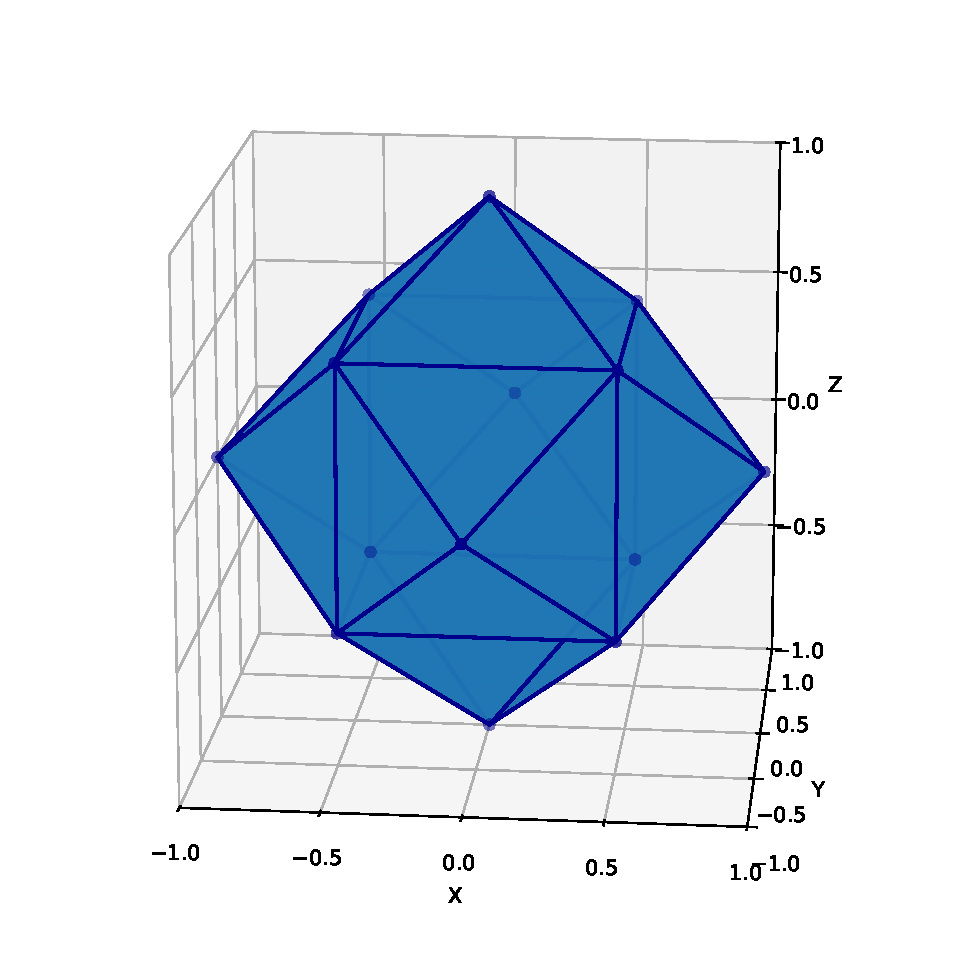
\includegraphics[width=\linewidth]{KyFan.pdf}
        \caption{Ky Fan 2-norm}
        \label{fig:kyfan}
    \end{subfigure}
    \hfill
    \begin{subfigure}[b]{0.45\linewidth}
        \centering
        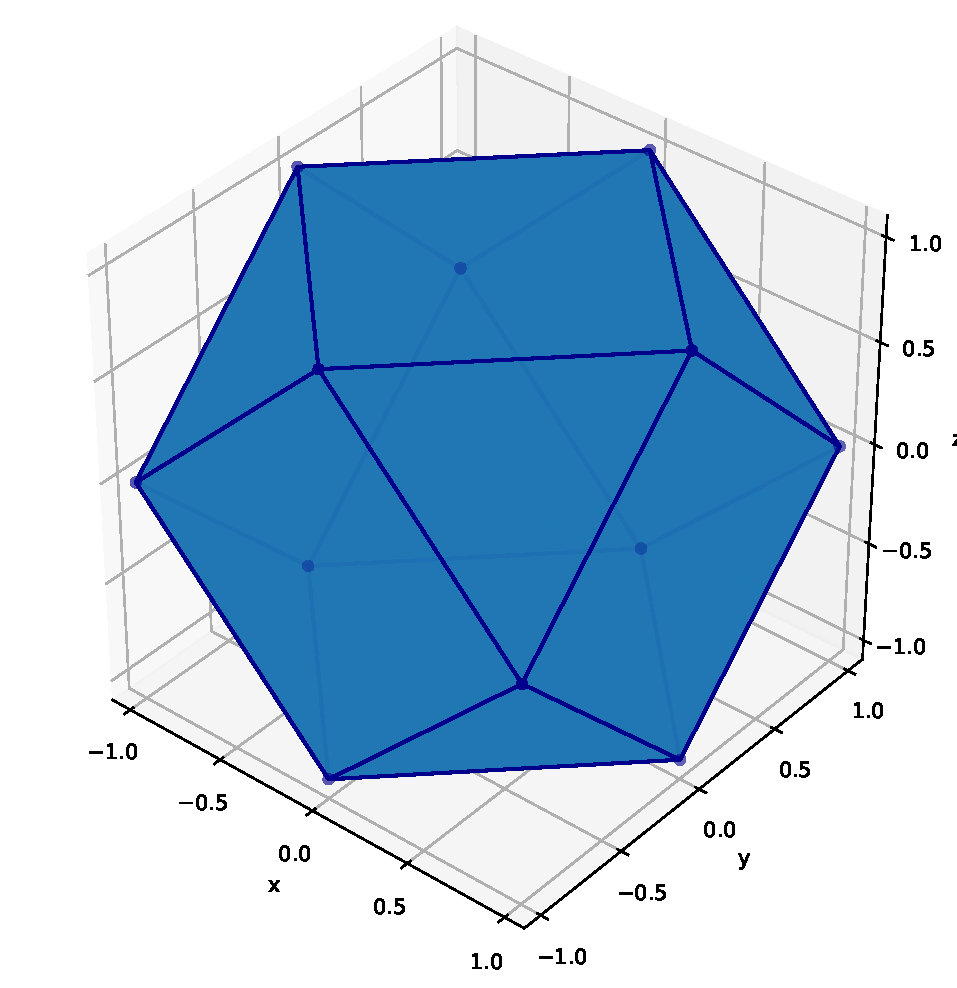
\includegraphics[width=\linewidth]{KyFanDual.pdf}
        \caption{Dual to Ky Fan 2-norm}
        \label{fig:kyfandual}
    \end{subfigure}
    \caption{Ky Fan 2-norm and its dual}
    \label{fig:kyfan_combined}
\end{figure}


\subsection{Updates derivations}

Proof of \cref{lemma:muon_update} follows from \cref{eq:nsgd_muon_update} with $\alpha=1$. Indeed, $\norms{\cdot}^\dagger=1\cdot\normn{\cdot} + 0 \cdot \normf{\cdot} $.

Proof of \cref{lemma:nsgd_muon_update}:
Since $\norm{\cdot}^\dagger = \normfstar{\cdot}^{\dagger\dagger} = \normfstar{\cdot}$, the goal is to reach $\normfstar{\mM^k} = \alpha \tr{\mSigma} + (1-\alpha) \normf{\mM^k}$.

Let us note that $\Delta = \alpha \mU \mV^\top + (1-\alpha) \frac{\mM^k}{\normf{\mM^k}}$ delivers this value. Indeed, by the trace property, $\<\mM^k, \Delta> =\<\mU \mSigma \mV^\top, \alpha \mU \mV^\top + (1-\alpha) \frac{\mU \mSigma \mV^\top}{\normf{\mM^k}}> = \alpha \tr \mSigma + (1-\alpha) \normf{\mM^k} = \normfstar{\mM^k}$, which completes the proof.

Proof of \cref{lemma:neon_update} follows from \cref{eq:nsgd_neon_update} with $\alpha=1$. Indeed, $\normn{\cdot}^\dagger=1\cdot\norms{\cdot} + 0 \cdot \normf{\cdot} $.

Proof of \cref{lemma:nsgd_neon_update}:
Since $\norm{\cdot}^\dagger = \normftwo{\cdot}^{\dagger\dagger} = \normftwo{\cdot}$, the goal is to reach $\normftwo{\mM^k} = \alpha \sigma_1 + (1-\alpha) \normf{\mM^k}$.

Let us note that $\Delta = \alpha (u_1 v_1^\top) + (1-\alpha) \frac{\mM^k}{\normf{\mM^k}}$ delivers this value. Indeed, by the trace property and singular vectors orthogonality, $\<\mM^k, \Delta> =\<\mU \mSigma \mV^\top, \alpha u_1 v_1^\top + (1-\alpha) \frac{\mU \mSigma \mV^\top}{\normf{\mM^k}}> = \alpha \tr \diag({\sigma_1, 0, \dots, 0}) + (1-\alpha) \normf{\mM^k} = \normftwo{\mM^k}$, which completes the proof.


Proof of \cref{lemma:ky_fan_update}:
Since $\norm{\cdot}^\dagger = \normkfk{\cdot}^{\dagger\dagger} = \normkfk{\cdot}$, the goal to reach $\normkfk{\mM^k}$.

Let us note that $\Delta = \sum_{i=1}^{k} u_i v_i^\top$ delivers the value. Indeed, $\<\mM^k, \Delta> =\<\mU \mSigma \mV^\top, \sum_{i=1}^{k} u_i v_i^\top> = \sum_{i,j=1}^{r, k}\<u_i \sigma_i v_i^\top, u_j v_j^\top> = \sum_{i=1}^{k}\sigma_i = \normkfk{\mM^k}$, which completes the proof. 

\subsection{Technical details of the experiments}


\iffalse

\section{Idea}
\iffalse
The goal of the project is to make variations on Muon to speed it up. Recently, authors of \cite{bernstein2024oldoptimizernewnorm} have proposed to derive update step for an optimizer as the solution of the certain optimization problem. This approach can be utilized to derive Muon \cite{jordan2024muon}, a novel algorithm for fast training of neural networks. Instead of using spectral norm, used to derive Muon, we utilize nuclear norm to produce a new optimization algorithm.
\fi
\subsection{Problem (Project description)}

In this subsection, we provide a more detailed description of our idea and formulate it as a mathematical problem. The authors of \cite{bernstein2024oldoptimizernewnorm} suggest obtaining the update step as a solution to the optimization problem:
\begin{equation}
    \langle g, \delta w \rangle + \lambda \norm{\delta w}^2 \to \min_{\delta w}\,,
\end{equation}
where $w$ is the weight vector, $g$ is a gradient-like vector (e.g., obtained via momentum SGD), and $\norm{\cdot}$ represents a certain norm. Many popular optimizers, such as Adam (with exponential moving average disabled) and vanilla SGD, can be cast within this framework \cite{bernstein2024oldoptimizernewnorm}.

In large language models, most weights are structured as matrices, which offers additional opportunities for optimization. Let $W$ be the weight matrix of a linear layer, and $G$ be a gradient-like matrix. Then, the update step $\delta W$ can be obtained as a solution to the optimization problem:
\begin{equation}\label{eqn:opt_problem_mat}
  \langle G, \delta W \rangle + \lambda \norm{\delta W}^2 \to \min_{\delta W}\,,
\end{equation}
where $\norm{\cdot}$ denotes a certain matrix norm. By setting this norm to the RMS-to-RMS norm (a scaled version of the spectral norm), we recover the Muon optimizer \cite{bernstein2025deriving, bernstein2024oldoptimizernewnorm} with an update step defined by:
\begin{equation}\label{eqn:update_muon}
\delta W = - \frac{1}{\lambda}\sqrt{\frac{n}{m}}UV^T\,,
\end{equation}
where $m$ is the input dimension of the layer, $n$ is the output dimension, and $U$ and $V$ are obtained from the singular value decomposition of the gradient matrix $G = U \Sigma V$.

Motivated by the recent achievements of the Muon optimizer (e.g., \cite{liu2025muon}), we consider alternative choices of norms, specifically the nuclear norm $\norm{\cdot}_*$ and a custom $F*$ norm, given by 
\begin{equation}\label{eqn:F_star}
    \norm{X}_{F*}^2 = \frac{\norm{X}_F^2 + \norm{X}_*^2}{2}\,,
\end{equation}
where $\norm{\cdot}_F$ denotes the Frobenius norm.

Using the nuclear norm in \eqref{eqn:opt_problem_mat} leads to a rank-one update of the weight matrices:
\begin{equation}\label{eqn:update_star}
  \delta W = -\frac{1}{2\lambda} u_1 \sigma_1 v_1^T\,,
\end{equation}
where $\sigma_1$ is the largest singular value, and $u_1$ and $v_1$ are the corresponding singular vectors. We expect one iteration of this method to be significantly faster than one iteration of Muon.

Another choice is the $F*$ norm. With this choice, \eqref{eqn:opt_problem_mat} yields 
\begin{equation}\label{eqn:update_F_star}
\delta W = -\frac{1}{\lambda}UDV^T
\end{equation} 
with $D = \text{diag}(d_i)$, where $d_i = [\sigma_i - \tau]_+$, and $\tau$ is given by
\begin{equation}
    \sum_{i} [\sigma_i - \tau]_+ = \tau\,.
\end{equation}
We anticipate that the method with this update step will perform well with large batch sizes.

In this article we show how one can quickly compute weight updates defined by \eqref{eqn:update_star} or \eqref{eqn:update_F_star}. Then we finilize the method by adding momentum and test their performance against those of Muon at training multilayer perceptron and transformer. The results will be fast algorithm, which we will convert into a new optimizer classes for PyTorch, as was done with Muon.

% Removed template instructions sections
\section{Related Work}
Our review primarily focuses on the Muon and Shampoo optimizers, as our algorithm extends the ideas used to derive these methods. We highlight the advantages and disadvantages of these approaches, the unique effects they introduce, and compare them to Neon.

\subsection{Muon optimizer}

In the previous section, we described the theoretical foundation behind the weight update step in the Muon optimizer, but we did not discuss how to obtain the required matrices in practice. The update step is defined by \eqref{eqn:update_muon}, which requires $UV^T$ with $U$ and $V^T$ from the singular value decomposition of the gradient-like matrix $G$. A naive solution would involve computing the SVD of $G$ and constructing the required expression. However, the developers of the Muon optimizer introduced a workaround using Newton-Schulz iterations \cite{jordan2024muon}. The Newton-Schulz iterations from the original article \cite{jordan2024muon} require 10 matrix-matrix multiplications to achieve the desired accuracy. The asymptotic complexity of such an operation is identical to that of SVD and equals $O(mn \min\{m, n\})$ for an $m \times n$ matrix. Nevertheless, matrix multiplication on modern GPUs can be performed much more efficiently.

The performance of Muon in training large language models was tested \cite{liu2025muon} against AdamW. The testing demonstrated excellent performance by Muon, which was approximately 2 times more efficient in terms of FLOPs required to reach a certain loss value. This is even more remarkable when considering the cost of one iteration: Muon requires an additional $O(mn \min\{m, n\})$ FLOPs per $m \times n$ matrix, while AdamW needs only $O(mn)$.

Another interesting discovery about the Muon optimizer is that it accelerates grokking \cite{tveit2025muonoptimizeracceleratesgrokking}. In the test problem, Muon achieved grokking significantly faster than AdamW in terms of passed epochs, with a mean grokking epoch of 102.89 for Muon and 153.09 for AdamW. The authors suggest that this may be due to the fact that Muon stimulates broader exploration by orthogonalizing the gradient matrix, thus avoiding memorization.

Recently, theoretical guarantees for Muon convergence have been derived \cite{li2025noteconvergencemuon}. In particular, in the $L$-smooth convex case, it achieves $O(1/T^{\frac{1}{2}})$ (with full gradient) and $O(1/T^{\frac{1}{4}})$ (with stochastic gradient) bounds on the Frobenius norm of the gradient or the mathematical expectation of the gradient norm, respectively, where $T$ is the number of iterations.

\subsection{Shampoo optimizer}

Another optimizer that exploits the matrix (and even tensor) structure of weights in neural networks is the Shampoo optimizer. We avoid a detailed description of this method here and refer the reader to the original article \cite{gupta2018shampoopreconditionedstochastictensor}, but we outline the key properties of Shampoo and its relation to the Muon optimizer.

The Shampoo optimizer uses left and right preconditioning for the gradient-like matrix, leveling its spectrum. The preconditioners are computed from the exponentially averaged gradients, and their computation requires $O(n^3 + m^3)$ per $m \times n$ matrix. This exponential averaging is a key feature that provides several distinct interpretations for the preconditioners. They can be viewed as an approximation of the Gauss-Newton component of the Hessian or the first step of the power iteration algorithm for computing the optimal Kronecker product approximation \cite{morwani2025a}. With exponential averaging turned off, the update step of Shampoo can be simplified and becomes identical to that of Muon \cite{jordan2024muon}.

Convergence analysis is presented in the original article \cite{gupta2018shampoopreconditionedstochastictensor}. Shampoo achieves $O(1/T^{\frac{1}{2}})$ convergence for the loss function value in the $L$-smooth convex case, where $T$ is the number of iterations.

\subsection{Synthesis and Neon's position}

Recent developments in optimization techniques show that utilizing the matrix structure of weights in neural networks can be very beneficial. Optimizers following this path converge faster in terms of iterations or epochs and often even FLOPs, but have a high iteration cost. Neon seeks to decrease the iteration cost while preserving fast convergence.

While the uniqie advantages and effects introduced by Neon are yet to be discovered, we can already say that our new optimizer introduces additional overhead of $O(mn)$ FLOPS on average per $m \times n$ weight matrix, which is much better then $O(m n \min\{m, n\})$ for Muon optimizer and $O(n^3 + m^3)$ for Shampoo. 

\subsection{Optimization Strategies for Efficient Large Language Model Training}
The unprecedented scale of modern Large Language Models (LLMs) has pushed traditional optimizers like AdamW \cite{Loshchilov2017FixingWD} to their limits in terms of computational efficiency and convergence speed \cite{liu2025muon,chen2025cosmoshybridadaptive}. This challenge has catalyzed research into more sophisticated optimization approaches that can maintain or improve performance while reducing training costs.

The Muon optimizer  has emerged as a promising alternative based on matrix orthogonalization principles. Scaling Muon to billion-parameter LLMs required two key adaptations: the integration of L2 weight decay for stability and the implementation of per-parameter update scaling to handle diverse parameter distributions efficiently . Empirical evaluations demonstrate that Muon can match or exceed AdamW's model quality while requiring only about 52 of the training FLOPs. The successful training of the Moonlight model series, including a 16B-parameter Mixture-of-Experts model, validates Muon's practicality for production-scale applications \cite{liu2025muon}.

Building on this foundation, hybrid approaches like COSMOS \cite{chen2025cosmoshybridadaptive} further enhance efficiency by combining optimization techniques based on gradient structure. COSMOS applies computationally intensive updates to a low-dimensional "leading eigensubspace" while using memory-efficient methods like Muon for the remaining parameters. This approach maintains convergence benefits while substantially reducing memory requirements. For distributed training environments, optimizers like Dion \cite{ahn2025dioncommunicationefficientoptimizerlarge} specifically target communication efficiency by minimizing data exchange between workers through distributed orthonormalization techniques.

\section{Derivation of update rules}

\begin{lemma}\label{lem:opt_star}
Let $G \in \mathbb{R}^{m \times n}$ and $\lambda > 0$. Then, the following optimization problem
\begin{equation*} 
  f(\delta W) = \langle G, \delta W \rangle + \lambda \norm{\delta W}_*^2 \to \min_{\delta W}
\end{equation*}
has solution 
\begin{equation*}
  \delta W = -\frac{1}{2\lambda} u_1 \sigma_1 v_1^T\,,
\end{equation*}
where $\sigma_1$ is the largest singular value of $G$, and $u_1$ and $v_1$ are the corresponding singular vectors.
\end{lemma}

\begin{proof}
Let us denote $r = \min\{m, n\}$. Then by Von Neumann's trace inequality,
\begin{equation*}
    \vert\langle G, \delta W \rangle\vert \leq \sum_{i=1}^r \sigma_i(G)\sigma_i(\delta W)
    \Rightarrow
    \langle G, \delta W \rangle \geq -\sum_{i=1}^r \sigma_i(G)\sigma_i(\delta W)\,.
\end{equation*}
Thus, expressing nuclear norm through singular values, we can write down
\begin{equation*}
    f(\delta W) \geq -\sum_{i=1}^r \sigma_i(G)\sigma_i(\delta W) + \lambda\left(\sum_{i=1}^{r}\sigma_i(\delta W)\right)^2 \geq \min_{d_1,\dots,d_r \geq 0}-\sum_{i=1}^r \sigma_i(G)d_i + \lambda\left(\sum_{i=1}^{r}d_i\right)^2.
\end{equation*}
By Karush-Kuhn-Tucker theorem, necessary conditions of minimum are
\begin{equation*}
    \left(d_i \geq 0\ \text{and}\ -\sigma_i(G) + 2\lambda\sum_{j=1}^{r}d_j = 0\right)\ \text{or}\ \left(d_i = 0\ \text{and}\ -\sigma_i(G) + 2\lambda\sum_{j=1}^{r}d_j \geq 0\right) \,\, i = 1,\dots,r\,.
\end{equation*}
These conditions simplify to 
\begin{equation*}
    \sum_{i \in S}d_i = \sigma_1(G)\,,\ \begin{cases}
        d_i \geq 0 & \text{if}\ \sigma_i(G) = \sigma_1(G)\,, \\
        d_i = 0 & \text{otherwise}\,.
    \end{cases}
\end{equation*}
All points satisfying those conditions deliver minimum, and
\begin{equation*}
    f(\delta W) \geq -\frac{\sigma_1^2(G)}{4\lambda}\,.
\end{equation*}

Now let
\begin{equation*}
    \delta W^* = -\frac{1}{2\lambda} u_1 \sigma_1(G) v_1^T\,.
\end{equation*}
Inserting it to $f(\delta W)$ gives
\begin{equation*}
    f\left(\delta W^*\right) = -\frac{\sigma_1(G)^2}{2\lambda} + \frac{\sigma_1(G)^2}{4\lambda} = -\frac{\sigma_1(G)^2}{4\lambda}
\end{equation*}
This matches the derived lower bound. Thus, $\delta W^*$ minimizes $f(\delta W)$.
\end{proof}

\begin{lemma}\label{lem:opt_F_star}
Let $G \in \mathbb{R}^{m \times n}$, $r = \min\{m. n\}$ and $\lambda > 0$. Then, the following optimization problem
\begin{equation*} 
  f(\delta W) = \langle G, \delta W \rangle + \lambda \norm{\delta W}_{F*}^2 \to \min_{\delta W}\,,
\end{equation*}
where $\norm{\cdot}_{F*}$ is defined in \eqref{eqn:F_star} has solution 
\begin{equation}
\delta W = -\frac{1}{\lambda}UDV^T
\end{equation} 
with $D = \text{diag}(d_i)$, where $d_i = [\sigma_i - \tau]_+$, and $\tau$ is given by
\begin{equation}
    \sum_{i=1}^r [\sigma_i - \tau]_+ = \tau\,.
\end{equation}
\end{lemma}

\begin{proof}
Analogously to the proof of Lemma~\ref{lem:opt_star}, we can use Von Neumann's trace inequality to write down
\begin{equation*}
    f(\delta W) \geq -\sum_{i=1}^r \sigma_i(G)\sigma_i(\delta W) + \frac{\lambda}{2}\left(\sum_{i=1}^{r}\sigma_i(\delta W)\right)^2 + \frac{\lambda}{2}\sum_{i=1}^{r}\sigma_i^2(\delta W)\,,
\end{equation*}
\begin{equation}\label{eqn:f_min_F_star}
    f(\delta W) \geq \frac{1}{\lambda}\min_{d_1,\dots,d_r \geq 0}-\sum_{i=1}^r \sigma_i(G)d_i + \frac{1}{2}\left(\sum_{i=1}^{r}d_i\right)^2 + \frac{1}{2}\left(\sum_{i=1}^{r}d_i^2\right)\,,
\end{equation}
By Karush-Kuhn-Tucker theorem, neccesary conditions of minimum are
\begin{equation*}
    \left(d_i \geq 0\ \text{and}\ -\sigma_i(G) + \sum_{j=1}^{r}d_j +  d_i = 0\right)\ \text{or}\ \left(d_i = 0\ \text{and}\ -\sigma_i(G) + \sum_{j=1}^{r}d_j + d_i \geq 0\right) \,\, i = 1,\dots,r\,.
\end{equation*}
Denoting $\tau = \sum_{i = 1}^r d_i$ gives $d_i = [\sigma_i(G) - \tau]_+$, where $\tau$ satisfies
\begin{equation}
    \sum_{i=1}^n [\sigma_i(G) - \tau]_+ = \tau\,.
\end{equation}
Inserting found minimum point into~\eqref{eqn:f_min_F_star} yields
\begin{equation*}
    f(\delta W) \geq -\sum_{i = 1}^r d_i(\tau + d_i) + \frac{\tau^2}{2\lambda} + \frac{1}{2\lambda}\sum_{i=1}^{r}d_i^2 = -\frac{1}{2 \lambda} \left( \tau^2 + \sum_{i=1}^r d_i^2 \right)\,.
\end{equation*}

Now let
\begin{equation}
\delta W^* = -\frac{1}{\lambda}UDV^T
\end{equation} 
with $D = \text{diag}(d_i)$. Inserting it to $f(\delta W)$ gives
\begin{equation*}
    f(\delta W^*) = -\sum_{i = 1}^r d_i(\tau + d_i) + \frac{\tau^2}{2\lambda} + \frac{1}{2\lambda}\sum_{i=1}^{r}d_i^2 = -\frac{1}{2 \lambda} \left( \tau^2 + \sum_{i=1}^r d_i^2 \right)\,.
\end{equation*}
This matches the derived lower bound. Thus, $\delta W^*$ minimizes $f(\delta W)$.
\end{proof}

\section{Quality metrics}
\begin{enumerate}
    \item The derivation is theoretically solid
    \item The numerical procedure used to compute a step is grounded and has estimated time overhead (say, in FLOPS)
    \item The code with Neon trains MLP and CNN (and NanoGPT, but it's a bonus) less than 3 times slower than Adam
    \item Instruction of setting the parameters of the algorithm are presented and justified
    \item The announced article has full structure (Abstract, Introduction, Theory, Experiments, Conclusion, Appendix)
    \item If results are positive, it is written with NeurIPS template.
\end{enumerate}

\section{Preliminary plan}
\paragraph{Week April 28 - May 4}
\begin{itemize}
    \item For Alexey: solve how to tune the algorithms for MLP and CNN, try formulating theory (and an appropriate model of the problem) why Muon and Neon are so successful, and create the drafts of the proofs. Register at NeurIPS site.
    
    \item For Ivan: write the theory for an update from the algebra point of view (as for an article)
    
    \item For Nikolay: write the theory for computing an update, and implement the method, if required
    
    \item For Alexander: reproduce results of Jordan on NanoGPT and ResNet (CIFAR-10), learn to train both models with Neon.
\end{itemize}

\paragraph{Week May 5 - May 11}
\begin{itemize}
    \item For Alexey: finalize the proofs. Verify them via small experiments on MLP and CNN. Write with Alexander Experiments for the article.
    
    \item For Ivan: join Nikolay to finalize algebra part of the article. Estimate FLOPS, memory and other overheads (produce O bounds)
    
    \item For Nikolay: write a draft of the poster (before May 6), and work with Ivan
    
    \item For Alexander: agressively test algorithms, prove that Neon outperforms competitors and prepare the results for the article.
    
    \item For everybody: write and edit the article
    
    \item May 11: submit an abstract to NeurIPS.
    
    \item May 12-14: the article is being polished.
    
    \item May 15: the article must be sent.
\end{itemize}

\section{Prototyping phase report}
\begin{enumerate}
    \item Update rule is derived, see idea
    \item Update rule methods are tested: power iteration vs Lanczos (see \ref{tab:matrix_methods})
    \item Recorded the distribution of singular values of gradients during NanoGPT training (see Firgures ~\ref{fig:svd_all}, \ref{fig:svd_all}).
    \begin{figure}[h!]
        \center{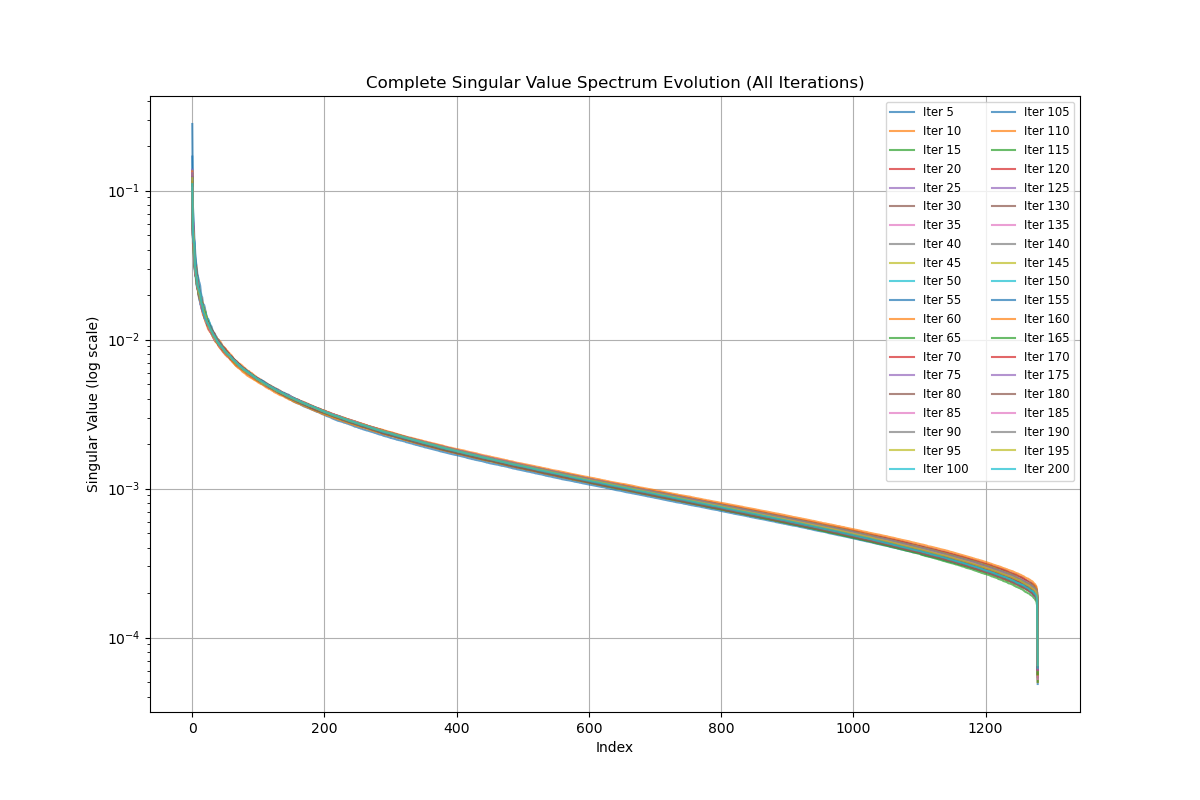
\includegraphics[width=0.8\linewidth]{figs/mlp24/svd_evolution_all.png}}
        \caption{Singular values of $50257\times 1280$ layer via 200 iterations}
        \label{fig:svd_all}
    \end{figure}
    \begin{figure}[h!]
        \center{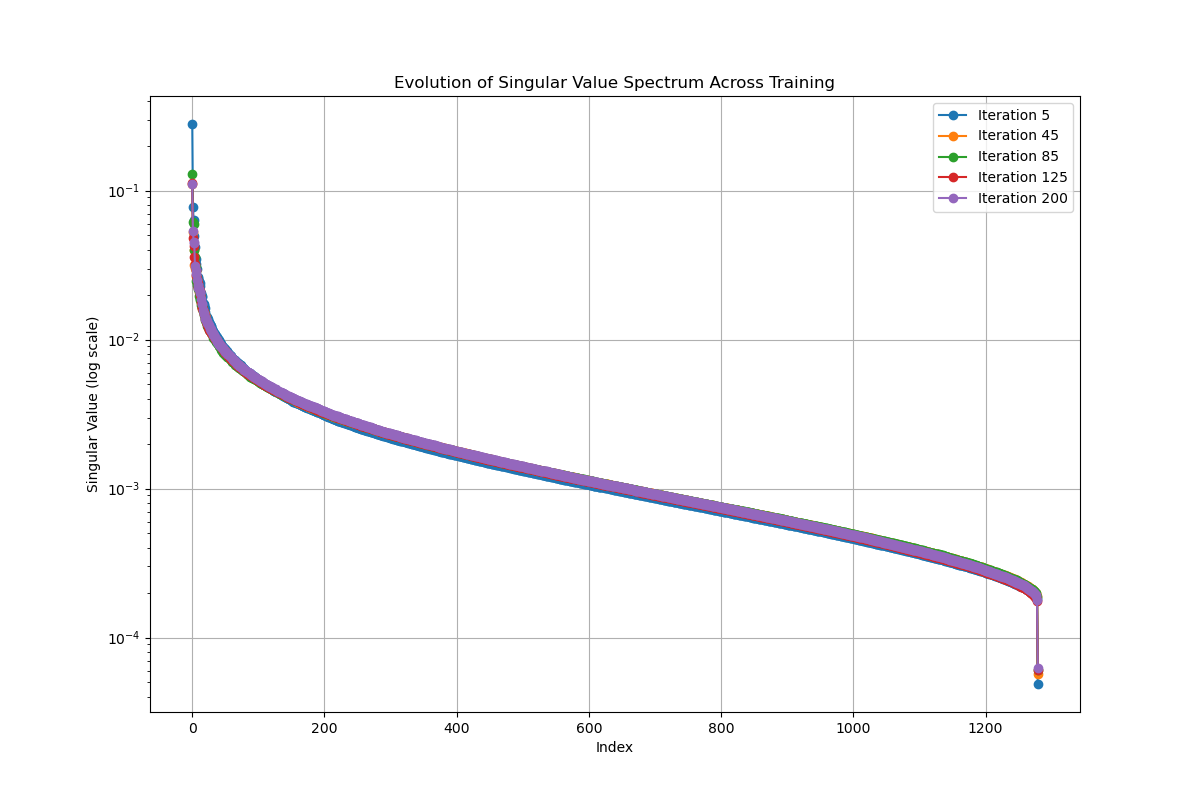
\includegraphics[width=0.8\linewidth]{figs/mlp24/svd_evolution.png}}
        \caption{Singular values of  of $50257\times 1280$ layer for 5-th,45-th, 65-th,175-th and 200-th iteration}
        \label{fig:svd}
    \end{figure} 
    
    \item NanoGPT is tested on Muon and Adam. For now, Neon (rank-1 version) does not converge (see Figures ~\ref{fig:train_loss} \ref{fig:val_loss})
    \begin{figure}[h!]
        \center{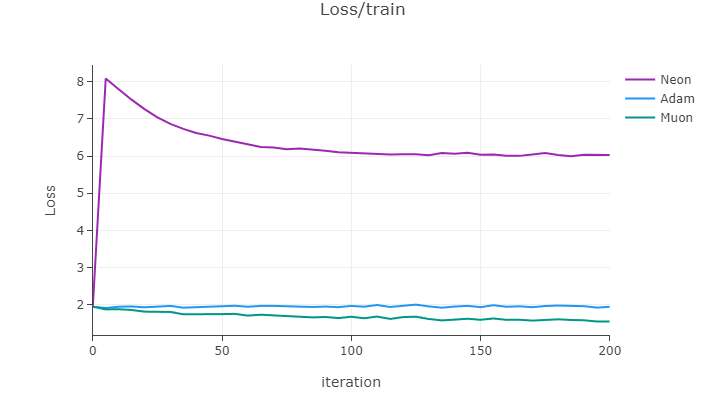
\includegraphics[width=0.8\linewidth]{figs/mlp24/loss_train.png}}
        \caption{Train loss}
        \label{fig:train_loss}
    \end{figure}
    \begin{figure}[h!]
        \center{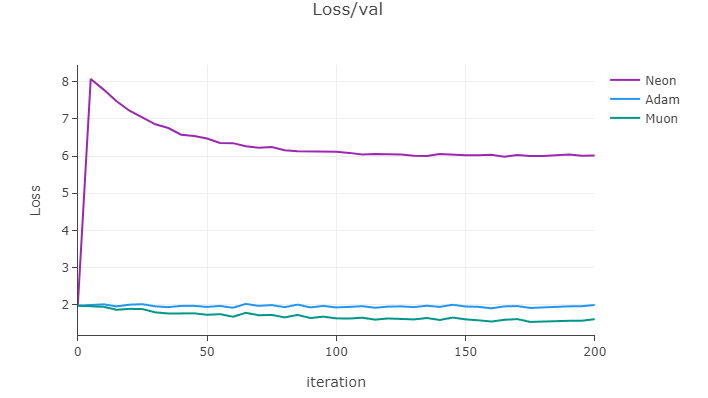
\includegraphics[width=0.8\linewidth]{figs/mlp24/loss_val.png}}
        \caption{Validation loss}
        \label{fig:val_loss}
    \end{figure} 


    The pictures show the best results achieved so far. The experiments were conducted with two 4090 24GB GPUs for nanotgpt-large on the tiny stories dataset.
    
    \item Neon (rank-1 version), Muon, AdamW and SGD are compared on MLP and CNN (see Figures~\ref{fig:mlp_epochs}, \ref{fig:cnn_epochs}, \ref{fig:mlp_time}, and~\ref{fig:cnn_time}). All methods work correctly, but again there is the problem with which one is the fastest (for now, it's SGD).
    \begin{figure}[h!]
        \center{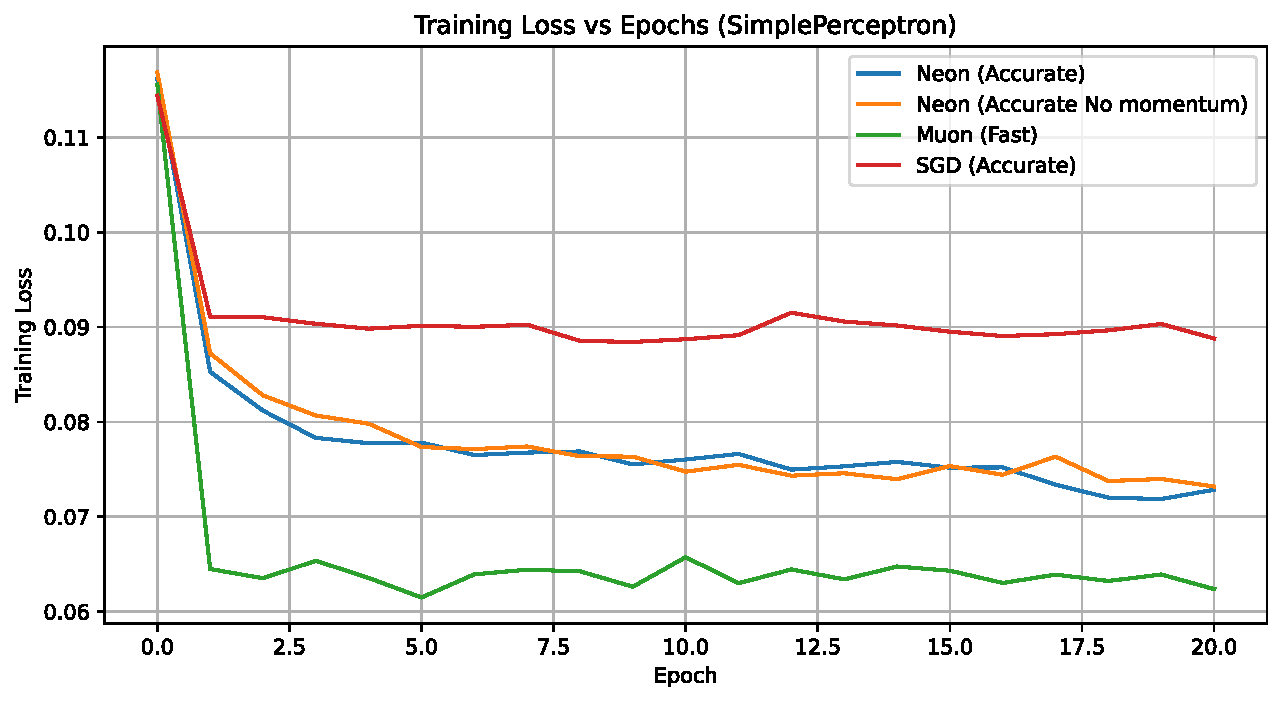
\includegraphics[width=0.8\linewidth]{figs/mlp0605/loss_vs_epochs_mlp.pdf}}
        \caption{MLP: self.linear1 = nn.Linear(32*32*3, 512), self.linear2 = nn.Linear(512, 10), self.activ = nn.GELU()}
        \label{fig:mlp_epochs}
    \end{figure}
    \begin{figure}[h!]
        \center{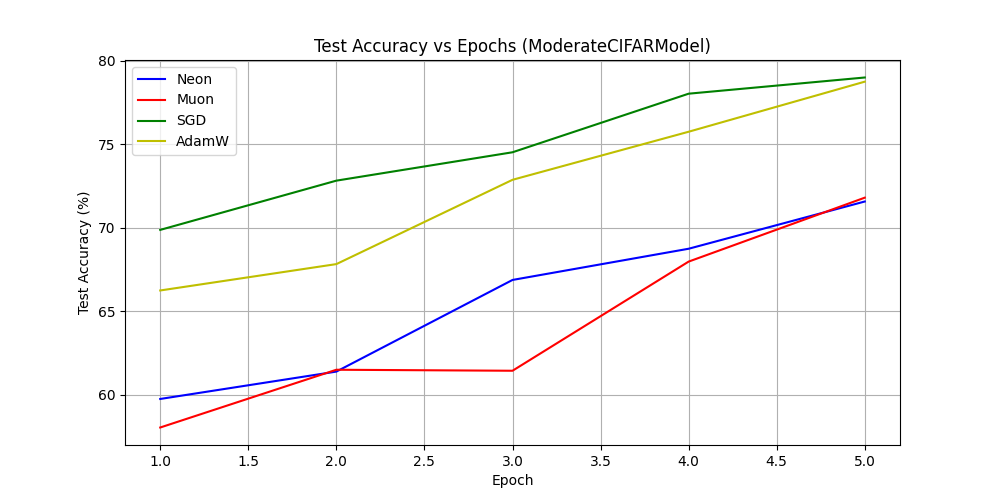
\includegraphics[width=0.8\linewidth]{figs/mlp24/accuracy_vs_epochs_moderate.png}}
        \caption{CNN: 2 convolutional blocks, 2 fully connected layers, activation + dropout}
        \label{fig:cnn_epochs}
    \end{figure}
    \begin{figure}[h!]
        \center{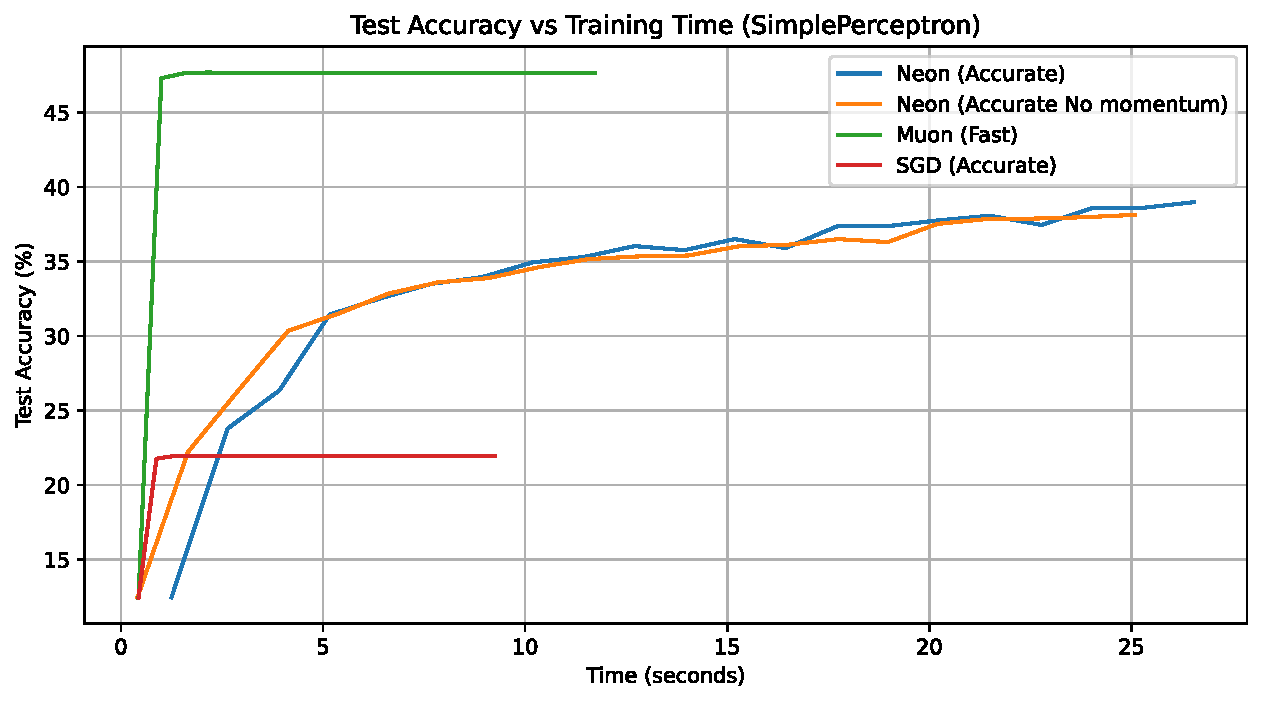
\includegraphics[width=0.8\linewidth]{figs/mlp0605/accuracy_vs_time_mlp.pdf}}
        \caption{MLP: wallclock time measurements}
        \label{fig:mlp_time}
    \end{figure}
    \begin{figure}[h!]
        \center{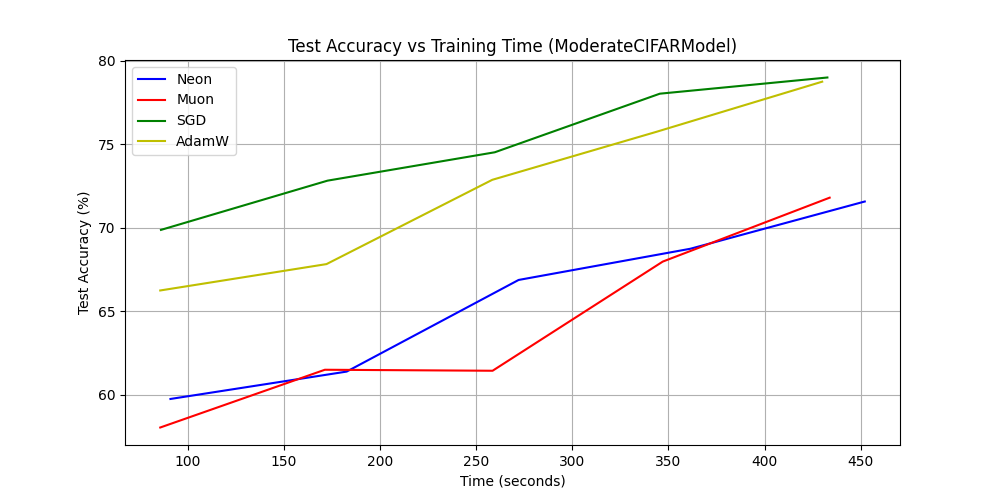
\includegraphics[width=0.8\linewidth]{figs/mlp24/accuracy_vs_time_moderate.png}}
        \caption{CNN: wallclock time measurements}
        \label{fig:cnn_time}
    \end{figure}
    \begin{table}[h!]
        \centering
        \begin{tabular}{c|c|c|c}
        \hline
        Method                              & rtol        & k & time,s \\
        \hline 
        Power Iterations                    & 0.01        & 1 & 7.7\\ 
        SVDS (thick-restart Lanczos method) & 0.01        & 1 & 0.18\\
        PCA Low Rank (RSVD)                 & 0.01        & 1 & 1.15\\
        SVDS (thick-restart Lanczos method) & 0.01        & 10 & 0.47\\
        PCA Low Rank (RSVD)                 & 0.01        & 10 & 19.4\\
        SVDS (thick-restart Lanczos method) & 0.01        & 100 & 1.96\\
        PCA Low Rank (RSVD)                 & 0.01        & 100 & 170\\
        \end{tabular}
        \caption{k-rank updated comparison}
        Comparison of different numerical methods to calculate k-rank update on $5000\times5000$ matrix of real numbers, rtol is an error in Frobenius norm relative to the k-rank approximation of truncated svd. During the research it was noted that rsvd can give good and fast approximation for singular values, but the matrix of approximation is far from the one given by truncated svd, while Lanczos method gives good and fast approximation for a matrix, but not so good approximation for singular values. 
        \label{tab:matrix_methods}
    \end{table}
\end{enumerate}


\appendix
\section{Old Appendix}
You may include other additional sections here.

\fi

\end{document}
